\documentclass[12pt]{article} 
%\usepackage{times,helvet}
\usepackage{palatino}
%\usepackage{ssss}
\usepackage{amsmath,amsbsy,amssymb}
\usepackage{sectsty,hangcaption}
%\usepackage{deflist}
\usepackage{fancyhdr}
\usepackage{tabularx}
\usepackage{verbatim}
\usepackage{moreverb}
\usepackage{float,comment}
\usepackage{graphicx}
\usepackage{longtable}
%\usepackage{portland}
\usepackage{booktabs}

%must be last package
%\usepackage{hyperref}
\usepackage[debug=false, colorlinks=true, pdfstartview=FitV, linkcolor=blue, citecolor=blue, urlcolor=blue, pdfpagelabels=true]{hyperref}

\textwidth 6.5in
\textheight 9.5in
%\topmargin -.1in
\topmargin -.75in
\newlength{\boxwidth}
\setlength{\boxwidth}{5.8in}
\oddsidemargin -0in
\evensidemargin -0in
\headheight 0.25in
\lhead{{\sl PFLOTRAN: Chemical Algorithms}}
\chead{\rm - \thepage\ -}
\rhead{\today}
\cfoot{}
\newcommand\flotran{{\sl FloTran}}
\renewcommand{\baselinestretch}{1.0}
\def\EQ#1\EN{\begin{equation}#1\end{equation}}
\def\BA#1\EA{\begin{align}#1\end{align}}
\def\BS#1\ES{\begin{split}#1\end{split}}
%\newcommand{\EQ}{\begin{equation}}
%\newcommand{\EN}{\end{equation}}
\newcommand{\bcr}{\begin{center}}
\newcommand{\ecr}{\end{center}}
\newcommand{\eq}{\ =\ }
\newcommand{\degc}{$^\circ$C}
\newcommand{\ecm}{{\rm ecm}}
\newcommand{\eff}{{\rm eff}}
\newcommand{\eqr}{{\rm le}}
\newcommand{\equ}{{\rm eq}}
\newcommand{\kin}{{\rm kin}}
\newcommand{\rdx}{{\rm rdx}}
\newcommand{\ind}{{\rm id}}
\newcommand{\dep}{{\rm dp}}
\newcommand{\e}{{\rm{e}}}
\newcommand{\erf}{{\rm{erf}}}
\newcommand{\erfc}{{\rm{erfc}}}
\newcommand{\p}{{\partial}}
\newcommand{\A}{{\mathcal A}}
\newcommand{\B}{{\mathcal B}}
\newcommand{\C}{{\mathcal C}}
\newcommand{\D}{{\mathcal D}}
\newcommand{\E}{{\mathcal E}}
\newcommand{\F}{{\mathcal F}}
\newcommand{\G}{{\mathcal G}}
\newcommand{\I}{{\mathcal I}}
\newcommand{\J}{{\mathcal J}}
\newcommand{\M}{{\mathcal M}}
\newcommand{\cO}{{\mathcal O}}
\renewcommand{\P}{{{\mathcal P}}}
\newcommand{\Q}{{\mathcal Q}}
\newcommand{\R}{{{\mathcal R}}}
\renewcommand{\S}{{\mathcal S}}
\newcommand{\T}{{\mathcal T}}
\newcommand{\W}{{\mathcal W}}
\newcommand{\Y}{{\mathcal Y}}
\newcommand{\Z}{{\mathcal Z}}
\newcommand{\rev}{{\rm rev}}
\newcommand{\irr}{{\rm irr}}
\renewcommand{\a}{{\alpha}}
\newcommand{\abar}{{\bar \alpha}}
\renewcommand{\b}{{\beta}}
\newcommand{\w}{{\rm H_2O}}
\newcommand{\air}{{\rm N_2}}
\newcommand{\pe}{{\rm Pe}}
\newcommand{\da}{{\rm Da}}
\renewcommand{\k}{{\dot R}^0}
\renewcommand{\L}{\widehat{\mathcal L}}
\renewcommand{\bar}{\overline}
\newcommand{\dsty}{{\displaystyle}}
\newcommand{\diff}{{\mathcal D}}
\newcommand{\surf}{\equiv \!\!\!}
\newcommand{\bnabla}{\boldsymbol{\nabla}}
\newcommand{\bA}{\boldsymbol{A}}
\newcommand{\ba}{\boldsymbol{a}}
\newcommand{\bB}{\boldsymbol{B}}
\newcommand{\bb}{\boldsymbol{\beta}}
\newcommand{\bC}{\boldsymbol{C}}
\newcommand{\bc}{\boldsymbol{c}}
\newcommand{\bcolon}{\boldsymbol{:}}
\newcommand{\bdot}{\boldsymbol{\cdot}}
\newcommand{\bD}{\boldsymbol{D}}
\newcommand{\bE}{\boldsymbol{E}}
\newcommand{\bF}{\boldsymbol{F}}
\newcommand{\bg}{\boldsymbol{g}}
\newcommand{\bi}{\boldsymbol{i}}
\newcommand{\bI}{\boldsymbol{I}}
\newcommand{\bJ}{\boldsymbol{J}}
\newcommand{\bK}{\boldsymbol{K}}
\newcommand{\bM}{\boldsymbol{M}}
\newcommand{\bn}{\boldsymbol{n}}
\newcommand{\bdelta}{\boldsymbol{\delta}}
\newcommand{\bGamma}{\boldsymbol{\Gamma}}
\newcommand{\bOmega}{\boldsymbol{\Omega}}
\newcommand{\bPsi}{\boldsymbol{\Psi}}
\newcommand{\bO}{\boldsymbol{O}}
\newcommand{\bnu}{\boldsymbol{\nu}}
\newcommand{\bdS}{\boldsymbol{dS}}
\newcommand{\bP}{\boldsymbol{P}}
\newcommand{\bq}{\boldsymbol{q}}
\newcommand{\br}{\boldsymbol{r}}
\newcommand{\bR}{\boldsymbol{R}}
\newcommand{\bS}{\boldsymbol{S}}
\newcommand{\bu}{\boldsymbol{u}}
\newcommand{\bv}{\boldsymbol{v}}
\newcommand{\bx}{\boldsymbol{x}}
\newcommand{\arrows}{~\rightleftharpoons~}
\newcommand{\arrowstab}{\!\!\!\rightleftharpoons\!\!\!}
\newcommand{\longline}{\noindent\rule[-0.1in]{\textwidth}{0.01in}}

%\numberwithin{equation}{section}

%\renewcommand{\theequation}{\arabic{section}.\arabic{equation}}

%\newcounter{saveeqn}%
%\newcommand{\seteqn}{\setcounter{saveeqn}{\value{equation}}%
%\stepcounter{saveeqn}\setcounter{equation}{0}%
%\renewcommand{\theequation}
%      {\mbox{\arabic{saveeqn}-\alph{equation}}}}%
%\newcommand{\reseteqn}{\setcounter{equation}{\value{saveeqn}}%
%\renewcommand{\theequation}{\arabic{equation}}}%

\newcounter{saveeqn}%
\newcommand{\seteqn}{\setcounter{saveeqn}{\value{equation}}%
\stepcounter{saveeqn}\setcounter{equation}{0}%
\renewcommand{\theequation}
      {\mbox{\arabic{section}.\arabic{saveeqn}\alph{equation}}}}%
\newcommand{\reseteqn}{\setcounter{equation}{\value{saveeqn}}%
\renewcommand{\theequation}{\arabic{section}.\arabic{equation}}}%

\setcounter{secnumdepth}{5}
\setcounter{tocdepth}{5}
%\renewcommand{\thepage}{\roman{page}}
%\renewcommand{\thepage}{\arabic{page}}
\renewcommand{\theequation}{\arabic{section}.\arabic{equation}}
%\setcounter{page}{1}

\setlength{\parindent}{0.3125in}
\setlength{\parskip}{2ex plus 0.2ex minus 0.2ex}

\renewcommand{\contentsname}{TABLE OF CONTENTS}
\setcounter{secnumdepth}{5}

\setlongtables

\pagestyle{fancy}

\thispagestyle{empty}

\begin{document}

\bcr

\section*{Chemistry Implementation in PFLOTRAN:}
\begin{tabular}{ll}
$\oplus$ & \bf\large Biogeochemistry with Monode Kinetics, \\
$\oplus$ & \bf\large Colloids,\\ 
$\oslash$&\bf\large Electrical Conductivity, \\
$\oslash$&\bf\large Hydration-Dehydration Reactions, \\
$\odot$ & \bf\large Ion Exchange, \\
$\oslash$&\bf\large Isotopic Exchange, \\
$\odot$ & \bf\large Multiphase Systems, \\
$\oplus$ & \bf\large Multiple Interacting Continua, \\
$\oslash$& \bf\large Pitzer Model, \\
$\odot$ & \bf\large Mineral Precipitation/Dissolution, \\
$\otimes$ & \bf\large Radioactive Decay Chain, \\
$\oslash$& \bf\large Solid Solutions, \\
$\oslash$& \bf\large Species-Dependent Diffusion, \\
$\otimes$ & \bf\large Stress-Strain\\
$\odot$ & \bf\large Surface Complexation (nonelectrostatic), \\
$\oplus$ & \bf\large Surface Complexation (electrostatic), \\
&\bf\large \ldots
\end{tabular}

\begin{tabular}{ll}\centering
$\odot$ & substantially completed\\
$\oplus$ & in progress\\
$\oslash$ & planned\\
$\otimes$ & not planned
\end{tabular}

\medskip

P.C. Lichtner (LANL, \today)

\ecr

\longline

\tableofcontents

\longline

\section{Reading the Thermodynamic Database}

\setcounter{equation}{0}

\subsection{Database Format}

The thermodynamic database stores all chemical reaction properties (equilibrium constant $\log K_r$, reaction stoichiometry $\nu_{ir}$, species valence $z_i$, Debye parameter $a_i$, mineral molar volume $\overline V_m$, and formula weight $w_i$) used in PFLOTRAN, with the exception of ion exchange. Reactions included in the database consist of aqueous complexation, mineral precipitation and dissolution, gaseous reactions, and surface complexation. The database is divided in five sections: database primary species, aqueous complex reactions, gaseous reactions, mineral reactions, and surface complexation. The format of the database is set up as shown in Table~\ref{tdatabase}. Equilibrium constants are stored at the temperatures: $\{$0, 25, 60, 100, 150, 200, 250, 300$\}$\degc. In the standard database the equilibrium constants are interpolated using a least squares fit to the Meier-Kelly expansion
\EQ
\log K \eq c_{-1} \ln T + c_0 + c_1 T + \frac{c_2}{T} + \frac{c_3}{T^2},
\EN
with coefficients $c_i$. As a consequence the entries in the database are not exactly reproduced at the corresponding temperatures. 

\begin{table}[h]\centering
\caption{Thermodynamic database format.}\label{tdatabase}
\vspace{3mm}
\begin{tabular}{ll}
\hline
Primary Species: & name, $a_0$, $z$, $w$\\
Secondary Species: & name, nspec, ($\nu$(n), name($n$), $n$=1, nspec), log$K$(1:8) $a_0$, $z$, $w$\\
Gaseous Species: & name, $\overline V$, nspec, ($\nu$(n), name($n$), $n$=1, nspec), log$K$(1:8), $w$ \\
Minerals: & name, $\overline V$, nspec, ($\nu$(n), name($n$), $n$=1, nspec), log$K$(1:8), $w$\\
Surface Complexes: & $>$name, nspec, $\nu$, $>$site, 
($\nu$(n), name($n$), $n$=1, nspec-1), log$K$(1:8), $z$, $w$\\
\hline
\end{tabular}
\end{table}

Redox reactions in the standard database are usually written in terms of O$_{2(g)}$.
Complexation reactions involving redox sensitive species are written in such a manner as to preserve the redox state.

\subsection{Primary Species: Transforming the Database}

The user must first select a set of aqueous primary species in terms of which the reactions in the database are then transformed. This is typically carried out as follows. For an arbitrary reaction corresponding to an aqueous complex that is read from the database with the form
\EQ
\varnothing\arrows\sum_i\nu_{ir}\A_i,
\EN
with $\varnothing$ representing the null species and equilibrium constant $K_r$. Partitioning the reacting species into primary and secondary species leading to the reaction
\EQ
\varnothing\arrows\sum_j\nu_{jr}\A_j + \sum_i\nu_{ir}\A_i.
\EN
Because, by construction, the matrix $\nu_{ir}$ is nonsingular, it can be inverted to give the canonical form
\EQ\label{canonical}
\sum_j\widetilde\nu_{ji}\A_j \arrows \A_i,
\EN
where
\EQ
\widetilde\nu_{ji} \eq -\sum_r\nu_{jr}(\nu^{-1})_{ri}.
\EN
These reactions are presumed to apply to both aqueous complexes and gaseous reactions. 
The equilibrium constant for reaction \ref{canonical} is given by
\EQ
\log K_i \eq \sum_r (\nu^{-1})_{ri} \log K_r.
\EN

For mineral reactions, the database form
\EQ
\sum_j\nu_{jm}\A_j + \sum_i\nu_{im}\A_i\arrows\M_m,
\EN
is transformed by eliminating the secondary species $\A_i$ using Eqn.\eqref{canonical} to give
\EQ
\sum_j\widetilde\nu_{jm}\A_j\arrows\M_m,
\EN
where
\EQ
\widetilde\nu_{jm}\eq\nu_{jm}+\sum_i\widetilde\nu_{ji}\nu_{im}.
\EN
The associated equilibrium constant $K_m'$ is given by
\EQ
\log K_m' \eq \log K_m + \sum_i \nu_{im}\log K_i.
\EN

\subsection{Distribution of Species Calculation}

Given various constraints imposed on an aqueous solution, the equilibrium concentration of all species in the system are determined. These constraints may consist of charge balance, mineral and gas equilibria, free ion concentration, pH, redox potential specified by Eh, pe, or $f_{\rm O_2}$, and total species concentration which may include sorption.

\subsubsection{Reaction Types}

\begin{description}

\item[Homogeneous]
\EQ
\sum_j\nu_{ji}\A_j\arrows\A_i.
\EN

\item[Heterogeneous: mineral]
\EQ
\sum_j\nu_{jm}\A_j\arrows\M_m.
\EN

\item[Heterogeneous: gas]
\EQ
\sum_j\nu_{ji}^g\A_j^{}\arrows\G_i.
\EN
\EQ
C_i^g \eq \frac{P_i}{RT} \eq \frac{K_i}{RT}\prod \left(\gamma_j m_j\right)^{\nu_{ji}^g}
\EN

\end{description}

\subsubsection{Constraint Conditions}

\begin{description}

\item[Total Concentration $\Psi_j^0$:]
\EQ
\Psi_j \eq \rho\big(m_j+\sum_i\nu_{ji} m_i\big) \eq \Psi_j^0.
\EN

\item[Total Sorbed Concentration $\Psi_j^0 + \frac{1}{\varphi}\sum_i\nu_{ji}^{\rm srf}(S_i^{\rm srf})_0 + \frac{1}{\varphi}\sum_i\nu_{ji}^{\rm ex}(S_i^{\rm ex})_0$:]
\BA
\Psi_j^{\rm tot} &\eq \Psi_j + \frac{1}{\varphi}\sum_i\nu_{ji}^{\rm srf}S_i^{\rm srf} 
+ \frac{1}{\varphi}\sum_i\nu_{ji}^{\rm ex}S_i^{\rm ex}\nonumber \\
&\eq \Psi_j^0 
+ \frac{1}{\varphi}\sum_i\nu_{ji}^{\rm srf}(S_i^{\rm srf})_0 
+ \frac{1}{\varphi}\sum_i\nu_{ji}^{\rm ex}(S_i^{\rm ex})_0.
\EA

\item[Free Ion: $m_j^0$]
\EQ
m_j \eq m_j^0.
\EN

\item[pH: $m_{\rm H^+}$]
\begin{subequations}
\BA
a_{\rm H^+} &\eq \gamma_{\rm H^+} m_{\rm H^+} \eq 10^{-\rm pH},\\
a_{\rm OH^-} &\eq \gamma_{\rm OH^-} m_{\rm OH^-} \eq K_{\rm H_2O} a_{\rm H_2O} 10^{\rm pH}.
\EA
\end{subequations}

\item[Charge Balance:]
\EQ
\Q \eq \sum_jz_j\Psi_j\eq \sum_j z_j m_j + \sum_i z_i m_i \eq 0.
\EN

\item[Mineral Equilibria:]
\begin{subequations}
\EQ
K_m \prod_j\left(\gamma_j m_j\right)^{\nu_{jm}}\eq 1,
\EN
\EQ
\ln K_m +\sum_j\nu_{jm}\ln\left(\gamma_j m_j\right)\eq 0.
\EN
\end{subequations}

\item[Gaseous Equilibria (Ideal Gas Law): $P_i$]
\begin{subequations}
\EQ
P_i \eq K_i \prod_j\left(\gamma_j m_j\right)^{\nu_{ji}^g},
\EN
\EQ
\ln P_i \eq \ln K_i+ \sum_j \nu_{ji}^g\ln\left(\gamma_j m_j\right).
\EN
\end{subequations}

\end{description}

\section{Homogeneous Reactions}

\setcounter{equation}{0}

Homogeneous reactions taking place within the aqueous phase can either be governed by local equilibrium relations or by kinetics as, for example, in sulfate reduction described by the reaction
\EQ
\rm SO_4^{2-} + H^+ - 2 O_{2(aq)} \arrows \rm HS^-. 
\EN
In this reaction sulfur is transformed through electron transfer from S$^{\rm VI}$ to S$^{-\rm II}$. Here it is necessary to ensure that complexes do not mix different redox states together. For example, the reactions
\EQ
\rm SO_4^{2-} + H^+ \arrows \rm HSO_4^-,
\EN
and
\EQ
\rm HS^- + H^+ \arrows \rm H_2S_{(aq)}.
\EN
preserve the sulfur redox state and can be consider to be in local equilibrium.

Local equilibrium reactions can always be written in the canonical form
\EQ
\sum_j\nu_{ji}\A_j \arrows \A_i.
\EN
Kinetic reactions depend on the specific mechanism and are assumed to have the general form
\EQ
\varnothing\arrows\sum_i\nu_{ir}\A_i.
\EN
Breaking this reaction out into primary and secondary species gives
\EQ
\varnothing\arrows\sum_j\nu_{jr}\A_j + \sum_i\nu_{ir}\A_i.
\EN
Eliminating the secondary species $\A_i$ yields the reactions
\EQ
\varnothing\arrows\sum_j\widetilde\nu_{jr}\A_j,
\EN
where
\EQ
\widetilde\nu_{jr} \eq \nu_{jr} + \sum_i \nu_{ji}\nu_{ir}.
\EN

The transport equations in the presence of homogeneous reactions take the form
\EQ
\frac{\p}{\p t} \varphi C_j + \bnabla\cdot\bF_j \eq -\sum_i\nu_{ji}I_i + \sum_r\widetilde\nu_{jr} I_r,
\EN
for primary species, and
\EQ
\frac{\p}{\p t} \varphi C_i + \bnabla\cdot\bF_i \eq I_i,
\EN
for secondary species. Noting that the rates $I_i$ for local equilibrium reactions are determined through algebraic mass action equations providing the concentrations of secondary species, these rates can be eliminated to yield the primary species transport equations
\EQ
\frac{\p}{\p t} \varphi \Psi_j + \bnabla\cdot\bOmega_j \eq \sum_r\widetilde\nu_{jr} I_r,
\EN
where the total concentration $\Psi_j$ is defined by
\begin{subequations}
\BA
\Psi_j &\eq C_j + \sum_i\nu_{ji}C_i,\\
&\eq\rho_w\big(m_j+\sum_i\nu_{ji}m_i\big),
\EA
\end{subequations}
where $C_l$ refers to the concentration in molarity units and $m_l$ in molality units. Molality $m_l$ is related to molarity $C_l$ by the expression
\BA
C_i &\eq \frac{n_i}{V_f} \eq \frac{n_i}{M_w}\frac{M_w}{M_f}\frac{M_f}{V_f},\\
&\eq m_i x_w\rho_f,
\EA
with fluid density $\rho_f\!=\!M_f/V_f$ and mole fraction $x_w\!=\!M_w/M_f$ of H$_2$O.
Since the fluid density is generally not known, an approximate expression
\EQ
C_l \simeq \rho_w m_l,
\EN
is used, where $\rho_w$ denotes the density of pure water and it is assumed that $x_w\simeq 1$. The activity of the $i$th secondary species is given by the relation
\EQ
a_i \eq K_i \prod_j\big(a_j\big)^{\nu_{ji}},
\EN
with equilibrium constant $K_i$, with activity $a_l = \gamma_im_l = \lambda_l C_l$. In terms of molality
\EQ\label{mi}
m_i \eq \gamma_i^{-1}K_i \prod_j \big(\gamma_j m_j\big)^{\nu_{ji}},
\EN
whereas in terms of molarity
\EQ
C_i \eq \lambda_i^{-1} K_i \prod_j\big(\lambda_j C_j\big)^{\nu_{ji}},
\EN
where the molarity-scale activity coefficients $\lambda_l$ are related to the molality-scale activity coefficients $\gamma_l$ approximately by
\EQ
\lambda_l \eq \frac{\gamma_l}{\rho_w}.
\EN

The total flux $\bOmega_j$ is defined by
\EQ
\bOmega_j \eq \bF_j + \sum_i\nu_{ji}\bF_i.
\EN
The flux $\bF_k$ has the usual form with contributions from advection and diffusion/dispersion given by
\EQ
\bF_k \eq \bq C_k - \varphi D \bnabla C_k,
\EN
with diffusion/dispersion coefficient $D$ assumed to be identical for all species. This condition is relaxed in the section below on species-dependent diffusion. For the case of equal diffusion coefficients the total flux becomes
\EQ
\bOmega_j \eq \big(\bq -\varphi D\bnabla\big) \Psi_j.
\EN

For low ionic strength electrolyte solutions, activity coefficients $\gamma_l$ are obtained from the Debye-H\"uckel algorithm
\EQ\label{dh}
\log\,\gamma_i \eq -\frac{z_i^2 A \sqrt{\I}}{1+B \stackrel{\circ}{a}_i \sqrt{\I}}+\dot b \I,
\EN
and the Davies algorithm defined by the expression
\EQ
\log\,\gamma_i \eq -\frac{z_i^2}{2}\left[\frac{\sqrt{\I}}{1+ \sqrt{\I}}-0.3 \I\right].
\EN
The ionic strength $\I$ is defined by
\EQ\label{ionic}
\I \eq \frac{1}{2} \sum_j z_j^2 m_j + \frac{1}{2} \sum_i z_i^2 m_i,
\EN
with molality $m_l$ and valence $z_l$. In the case of the Debye-H\"uckel and Davies algorithms, the activity coeffients are determined by solving a nonlinear equation for the ionic strength.
For high ionic strength solutions, the Pitzer model must be used which is described in a later section.

\subsection{Debye-H\"uckel Activity Coefficient Algorithm}

For the Debye-H\"uckel model the activity coefficients are functions of the ionic strength $\I$ according to Eqn.\eqref{dh}. The ionic strength, in turn, is a function of the activity coefficients according to the definition Eqn.\eqref{ionic}. This relation defines a nonlinear equation to determine the ionic strength and hence the activity coefficients according to
\BA\label{f}
g(\I) &\eq \frac{1}{2} \sum_j z_j^2 m_j + \frac{1}{2} \sum_i z_i^2 m_i(\I) -\I,\\
&\eq f(\I)-\I.
\EA
The ionic strength is obtained through Newton-Raphson iteration to give
\BA
\I_{k+1} &\eq \I_k-\dfrac{g(\I_k)}{\dfrac{dg(\I_k)}{d\I}},\\
&\eq \I_k - \dfrac{f(\I_k)-\I_k}{f_k'-1} \eq \dfrac{f_k-\I_k f_k'}{1-f_k'},
\EA
for the $k+1$st iteration. From Eqn.\eqref{f}
\EQ
\frac{df}{d\I}\eq \frac{1}{2} \sum_i z_i^2 \frac{dm_i(\I)}{d\I} -1,
\EN
where, differentiating the logarithm of Eqn.\eqref{mi} for the $i$ secondary species gives
\EQ
\frac{1}{m_i}\frac{dm_i}{d\I} \eq -\frac{1}{\gamma_i}\frac{d\gamma_i}{d\I} + \sum_j\nu_{ji}\frac{1}{\gamma_j}\frac{d\gamma_j}{d\I}.
\EN
It follow from Eqn.\eqref{dh} that
\EQ
\frac{1}{\gamma_i}\frac{d\gamma_i}{d\I}\eq \frac{1}{2} \frac{z_i^2 A \I^{-1/2}}{\left(1+\stackrel{\circ}{a}_i B\sqrt{\I}\right)^2} + \dot b.
\EN

\subsection{Jacobian}

To construct the Jacobian matrix the following derivatives are needed
\EQ
\frac{\p\Psi_j}{\p m_l} \eq \delta_{jl} + \frac{1}{m_l}\sum_i\nu_{ji}\nu_{li}m_i.
\EN
The logarithmic derivatives are symmetric thereby reducing storage
\EQ
\frac{\p\Psi_j}{\p \ln m_l} \eq m_j\delta_{jl} + \sum_i\nu_{ji}\nu_{li}m_i \eq \frac{\p\Psi_l}{\p \ln m_j}.
\EN
Finally, the stoichiometric has zero elements and may be reduced in size through compression.

\section{Mineral Precipitation/Dissolution Reactions}

\setcounter{equation}{0}

Mineral precipitation/dissolution reactions are assumed to have the form
\EQ
\sum_j\nu_{jm}\A_j \arrows \M_m.
\EN
The rate law based on transition state theory has the general form
\BA\label{ratemin}
\widehat I_m &\eq - {\rm sgn}_m s_m^{} \left(\sum_l \P_{ml}^{} k_{ml}^{} \right) \bigg| 1- \left(K_m Q_m\right)^\frac{1}{\sigma_m} \bigg|^{\beta_m},\\
&\eq - {\rm sgn}_m s_m^{} \left(\sum_l \P_{ml}^{} k_{ml}^{} \right) \bigg| 1- \e^{-A_m/(\sigma_mRT)} \bigg|^{\beta_m},
\EA
where the affinity $A_m$ is defined as
\EQ
A_m \eq -RT\ln K_mQ_m,
\EN
the quantity sgn$_m$ denotes the sign of the affinity factor
\EQ
{\rm sgn}_m \eq \dfrac{1- \left(K_m Q_m\right)^{1/\sigma_m}}{\big| 1- \left(K_m Q_m\right)^{1/\sigma_m}\big|},
\EN
where $K_m$ represents the equilibrium constant, $Q_m$ denotes the ion activity product
\EQ
Q_m\eq\prod_j\big(\gamma_j m_j\big)^{\nu_{jm}},
\EN
the prefactor $\P_{ml}$ is defined as the product of contributions from primary and secondary species:
\EQ\label{prefactorm}
\P_{ml} \eq \left[\prod_{j=1}^{N_c} \frac{a_j^{\alpha_{jl}^m}}{1+K_{jl}^{} a_j^{\beta_{jl}^m}} \right] \,
\left[\prod_{i=1}^{N_{cx}} \frac{a_i^{\alpha_{il}^m}}{1+K_{il}^{} a_i^{\beta_{il}^m}}\right],
\EN
$k_{ml}$ denotes the kinetic rate constant for the $l$th parallel reaction, $s_m$ denotes the specific mineral surface area participating in the reaction, $\sigma_m$ denotes Tempkin's constant, $a_i$ represents the activity of the $i$th species, and $\alpha_{jl}^m$, $\alpha_{il}^m$ are a constants. A transport-limited form of the rate law can be devised according to the expression
\EQ\label{ratemintran}
\widehat I_m \eq -s_m^{} \sum_l \P_{ml}^{} k_{ml}^{} \left[ \dfrac{1-\left(K_m Q_m\right)^{1/\sigma_m}}{1+\dfrac{k_{ml}^{}}{r_m^{\rm lim}} \left(K_m Q_m\right)^{1/\sigma_m}} \right],
\EN
with transport-limited rate $r_{\rm lim}$. In the limit $K_mQ_m\rightarrow\infty$, the rate becomes
\EQ
\lim_{K_mQ_m\rightarrow\infty}\widehat I_m \eq r_m^{\rm lim} s_m^{}\sum_l \P_{ml}^{}.
\EN

Adding mineral precipitation/dissolution to the mass conservation equations yields
\EQ
\frac{\p}{\p t} \varphi \Psi_j + \bnabla\cdot\bOmega_j \eq \sum_r\widetilde\nu_{jr}I_r -\sum_m \nu_{jm} I_m,
\EN
\EQ
\frac{\p\varphi_m}{\p t} \eq \overline V_m I_m.
\EN

\section{Sorption}

\setcounter{equation}{0}

\subsection{Surface Complexation Reactions}

\noindent
Surface complexation reactions are assumed to have the general form
\EQ
\nu_i^\a >\!\!\!X_\a + \sum_j \nu_{ji}^\a \A_j \arrows >\!\!\!\A_i^\a,
\EN
for surface complex $>\!\!\!\A_i^\a$ and empty surface site $>\!\!\!X_\a$ on surface sites designated by $\a$. Each surface site $\a$ corresponds to a particular type of site $s_m$ associated with a particular mineral $\M_m$. Thus $\a = (m,\,s_m)$ can be represented by two indices $m$ and $s_m$. Conservation of surface sorption sites is expressed as
\EQ
\omega_\a = S_X^\a + \sum_i \nu_i^\a S_i^\a,
\EN
where the surface site concentration $\omega_\a$ is given by
\EQ
\omega_\a \eq \frac{N_\a}{V} \eq \frac{N_\a}{A_m}\frac{A_m}{M_m}\frac{M_m}{V_m}\frac{V_m}{V} \eq \eta_m^\a \A_m \rho_m \varphi_m.
\EN
Based on bulk rock properties the site concentration is expressed as
\EQ
\omega_\a \eq \frac{N_\a}{V} \eq \frac{N_\a}{A_s}\frac{A_s}{M_s}\frac{M_s}{V_s}\frac{V_s}{V} \eq \eta_s^\a \A_s \rho_s (1-\varphi).
\EN

The mass conservation equations in the presence of surface complexation reactions have the form
\BA
\frac{\p}{\p t} \varphi \Psi_j + \bnabla\cdot\bOmega_j &= -\sum_{i\a} \nu_{ji}^\a I_i^\a -\sum_m\nu_{jm}I_m,\\
\frac{\p S_i^\a}{\p t} &= I_i^\a,\\
\frac{\p S_X^\a}{\p t} &= -\sum_{i} \nu_{i}^\a I_i^\a.
\EA
Eliminating the reaction rates $I_i^\a$ leads to the equations
\EQ\label{transsorp}
\frac{\p}{\p t} \left\{\varphi \Psi_j +\sum_{i\a} \nu_{ji}^\a S_i^\a \right\} + \bnabla\cdot\bOmega_j \eq -\sum_m\nu_{jm}I_m.
\EN

The sorption reaction rate $I_i^\a$ expressed as an elementary reaction has the form
\EQ
I_i^\a = k_i^{\a f} (S_X^\a)^{\nu_i^\a} \prod_j a_j^{\nu_{ji}^\a} - k_i^{\a b} S_i^\a,
\EN
with forward and backward rate constants $k_i^{\a f}$ and $k_i^{\a b}$, respectively.

\subsubsection{Site Conservation}

Note that the sorption site concentration $\omega_\a$ is conserved with respect to surface complexation reactions:
\EQ
\left(\frac{\p\omega_\a}{\p t}\right)_{\rm \tiny\hspace{-8pt}
\begin{array}{c}
surf.\\
cmplx
\end{array}
}
\eq \frac{\p S_X^\a}{\p t} + \sum_i\nu_i^\a \frac{\p S_i^\a}{\p t} \eq 0.
\EN
However, precipitation/dissolution reactions can lead to a change in $\omega_\a$:
\BA
\left(\frac{\p\omega_\a}{\p t}\right)_{\rm \tiny\hspace{-8pt}
\begin{array}{c}
precip.\\
/diss.
\end{array}
} 
&\eq \eta_m^\a\A_m^{}\rho_m^{}\frac{\p\varphi_m}{\p t},\\
&\eq \eta_m^\a\A_m^{}\rho_m^{}\overline V_m^{} I_m^{}.
\EA

\subsubsection{Charge Conservation}

Charge is generally {\em not} conserved by the continuum transport equations Eqns.\eqref{transsorp}. Multiplying this equation through by the valence $z_j$ of the $j$th primary species and summing gives
\EQ
\frac{\p}{\p t} \left\{\varphi \sum_j z_j\Psi_j +\sum_{ji\a} z_j\nu_{ji}^\a S_i^\a \right\} + \bnabla\cdot\sum_jz_j\bOmega_j \eq -\sum_{jm} z_j\nu_{jm}I_m.
\EN
Noting that
\EQ
\sum_j z_j\nu_{jm}\eq 0,
\EN
and
\EQ
\sum_j z_j \nu_{ji}^\a \eq z_i,
\EN
assuming empty surface sites have zero valence, and defining the charge density $\rho_Q \!=\!\F\sum_j z_j\Psi_j$ with Faraday constant $\F$, gives
\EQ\label{chrgconv}
\frac{\p}{\p t} \left\{\varphi \rho_Q +\sum_{i\a} z_i S_i^\a \right\} + \bnabla\cdot\bJ_\Q \eq 0,
\EN
where the current density $\bJ_\Q$ is given by
\EQ
\bJ_Q \eq \F\bq \rho_Q.
\EN
Alternatively, Eqn.\eqref{chrgconv} can be written in the form
\EQ
\frac{\p}{\p t} \left(\varphi \rho_Q \right) + \bnabla\cdot\bJ_\Q \eq -\F\sum_{i\a} z_i S_i^\a,
\EN
and thus charge is conservation only if the right-hand side vanishes.

\subsubsection{Electric Double Layer}

Diffuse layer concentration $C_i^m$ associated with the surface of the $m$th mineral is related to the bulk concentration $C_i^b$ through the Boltzmann factor
\EQ
C_i^m(x) \eq C_i^b \, \e^{-z_i F \Phi_m(x)/RT},
\EN
where $\Phi_m$ denotes the electric potential resulting from sorption on the surface of the $m$th mineral. The potential satisfies the Poisson equation
\EQ
\frac{d^2 \Phi_m}{dx^2} \eq - \frac{1}{\epsilon \epsilon_0} \rho_m (x).
\EN
In this equation $\epsilon_0$ denotes the permitivity of free space, $\epsilon$ represents the dielectric constant of pure water, and $\rho_m$ refers to the charge density of the diffuse layer defined by
\EQ
\rho_m^{} (x) \eq F \sum_i z_i^{} C_i^m.
\EN

\begin{table}[H]\centering
\caption{Fundamental constants at 25\degc.}

\vspace{4mm} 

\begin{tabular}{lcc}
\hline
$N_A$ & $6.023 \times 10^{23}$& mol$^{-1}$\\
$\epsilon$ & 78.5&\\
$\epsilon_0$ & $8.854 \times 10^{-14}$ & ${\rm Coul}/({\rm V cm})$\\
$F$ & 96485 & ${\rm Coul}/{\rm mol}$\\
\hline
\end{tabular}
\end{table}

The sorbed surface charge $\sigma_m$ is related to the bulk concentration and potential by the expression
\EQ
\sigma_m^{} \eq \sqrt{2 \epsilon \epsilon_0 RT \sum_i C_i^b \left(\e^{-z_i F\Phi_m^0 /RT}-1\right)},
\EN
where $\Phi_m^0$ denotes the value of the potential at the mineral surface.
For a $z\!\!:\!\!z$ electrolyte with concentration $C_0$ the expression for the surface charge reduces to
\EQ
\sigma_m^{} \eq \sqrt{8\epsilon \epsilon_0 RT C_0} \, {\rm sinh} \left[\frac{zF\Phi_m^0}{RT}\right].
\EN
This result is obtained from the identity
\EQ
{\rm sinh} \left[\frac{x}{2}\right] \eq \frac{1}{2} \sqrt{\e^x+\e^{-x}-2}.
\EN

The volumetric sorbed charge density $q_m$ is given by the sum of sorbed ion concentrations multiplied by their respective valencies as
\EQ
q_m^{} \eq F\sum_{s\alpha} z_{s\alpha}^m \overline C_{s\alpha}^m,
\EN
where the sum is taken over all sorbed species on all sorption sites corresponding to the $m$th mineral.
The relation between volumetric charge density $q_m$ and surface charge density $\sigma_m$ can be derived as follows
\BA
q_m^{} &= \frac{Q_m}{V},\nonumber\\
&= \frac{Q_m}{A_m} \, \frac{A_m}{M_m} \, \frac{M_m}{N_m} \, \frac{N_m}{V_m} \, \frac{V_m}{V},\nonumber\\
&= \sigma_m^{} \A_m^{} W_m^{} \overline V_m^{-1} \phi_m^{}.
\EA
Therefore
\EQ
\sigma_m^{} \eq \dfrac{Q_m^{}}{A_m^{}} \eq \dfrac{q_m^{}}{\A_m^{} W_m^{} \overline V_m^{-1} \phi_m^{}}.
\EN

In the presence of the electric double layer potential the unoccupied site concentration $\overline C_\alpha^m$ becomes
\EQ
\overline C_\alpha^m \eq \frac{\omega_\alpha^m}{1+\sum_s K_{s\alpha}^m \prod_j \left(\gamma_j C_j \P^{z_j} \right)^{\nu_{js}^{m\alpha}}},
\EN
and the sorbed concentration is given by
\EQ
\overline C_{s\alpha}^m \eq \frac{\omega_\alpha^m K_{s\alpha}^m \prod_j \left(\gamma_j C_j \P^{z_j} \right)^{\nu_{js}^{m\alpha}}}{1+\sum_{s'} K_{s'\alpha}^m \prod_j \left(\gamma_j C_j \P^{z_j} \right)^{\nu_{js'}^{m\alpha}}},
\EN
where the factor $\P$ is defined by
\EQ
\P \eq \e^{-F \Phi_m^0/RT}.
\EN
Noting that
\EQ
\prod_j \P^{z_j^{}\nu_{js}^{m\alpha}} \eq \P^{\sum_j z_j^{} \nu_{js}^{m\alpha}} \eq \P^{z_{s\alpha}^m},
\EN
using the identity
\EQ
\sum_j z_j^{} \nu_{js}^{m\alpha} \eq z_{s\alpha}^m,
\EN
these relations become
\EQ
\overline C_\alpha^m \eq \frac{\omega_\alpha^m}{1+\sum_s K_{s\alpha}^m \P^{z_{s\alpha}^m} \prod_j \left(\gamma_j C_j \right)^{\nu_{js}^{m\alpha}}},
\EN
and the sorbed concentration is given by
\EQ
\overline C_{s\alpha}^m \eq \frac{\omega_\alpha^m K_{s\alpha}^m \P^{z_{s\alpha}^m} \prod_j \left(\gamma_j C_j \right)^{\nu_{js}^{m\alpha}}}{1+\sum_{s'} K_{s'\alpha}^m \P^{z_{s'\alpha}^m} \prod_j \left(\gamma_j C_j \right)^{\nu_{js'}^{m\alpha}}}.
\EN

In the presence of the electric double layer potential the expression for the kinetic reaction rate based on a pseudo-kinetic description of sorption takes the form
\EQ
I_{s\alpha}^m \eq k_{s\alpha}^{fm} \dfrac{\omega_\alpha^m \P^{z_{s\alpha}^m} \prod_j a_j^{\nu_{js}^{m\alpha}}}{1+\sum_{s'} K_{s'\alpha}^m \P^{z_{s'\alpha}^m} \prod_j a_j^{\nu_{js'}^{m\alpha}}} - k_{s\alpha}^{bm} \overline C_{s\alpha}^m.
\EN

The potential at the $m$th mineral surface may be obtained by solving a nonlinear equation equating the diffuse layer charge to the sorbed charge. Substituting for $q_m$ the surface charge density can be expressed as
\EQ
\sigma_m \eq \frac{F}{N_A} \sum_\alpha \frac{\eta_\alpha^m}{\D_\alpha^m} \sum_s z_{s\alpha}^m K_{s\alpha}^m \P^{z_{s\alpha}^m} \prod_j a_j^{\nu_{js}^{m\alpha}},
\EN
where
\EQ
\D_\alpha^m \eq 1+\sum_s K_{s\alpha}^m \P^{z_{s\alpha}^m} \prod_j a_j^{\nu_{js}^{m\alpha}}.
\EN
With this result the following equation is obtained for the potential
\BA
f(\Phi_m^0) &= \sqrt{\sum_i C_i^b \left(\P^{z_i}-1\right)} - \frac{\sigma_m}{\sqrt{2 RT\epsilon \epsilon_0}},\nonumber\\
&=\sqrt{\sum_i C_i^b \left(\P^{z_i}-1\right)} - \frac{1}{\sqrt{2 RT\epsilon \epsilon_0}} \left[\frac{1}{N_A} \sum_\alpha \frac{\eta_\alpha^m}{\D_\alpha^m} \sum_s z_{s\alpha}^m K_{s\alpha}^m \P^{z_{s\alpha}^m} \prod_j a_j^{\nu_{js}^{m\alpha}} \right],\nonumber \\
&=0.
\EA
Setting $\xi = F\Phi_m^0/RT$, the Jacobian is found to be
\EQ
\frac{df}{d \xi} \eq -\dfrac{\sum_i z_i C_i^b \P^{z_i}}{2 \sqrt{\sum C_i^b P^{z_i}}} - \frac{1}{\sqrt{2RT\epsilon \epsilon_0}} \, \frac{d\sigma_m}{d\xi},
\EN
with
\BA
\frac{d\sigma_m}{d\xi} &= -\frac{F}{N_A} \sum_\alpha \frac{\eta_\alpha^m}{\D_\alpha^m} \left\{\rule[0mm]{0mm}{9mm} \sum_s (z_{s\alpha}^m)^2 K_{s\alpha}^m \P^{z_{s\alpha}^m} \prod_j a_j^{\nu_{js}^{m\alpha}} \right. \nonumber\\
&\qquad\qquad \left. - \frac{1}{\D_\alpha^m} \left(\sum_s z_{s\alpha}^m K_{s\alpha}^m \P^{z_{s\alpha}^m} \prod_j a_j^{\nu_{js}^{m\alpha}} \right)^2 \rule[0mm]{0mm}{9mm} \right\}.
\EA
The potential is computed from the Newton-Raphson algorithm
\EQ
\xi_{k+1} \eq \xi_k - \frac{f_k}{df_k/d\xi}.
\EN

\subsubsection{Bulk Properties}

In many cases surface complexation properties are specified in terms of bulk properties of the porous medium: $\eta_b$, $\A_b$, $\rho_b$, $\varphi$. To represent this situation a fictitious mineral $\M_{m_0}$ may be entered with properties that reproduce the bulk density of the system by taking $W_{m_0}^{}\overline V_{m_0}^{-1}\varphi_{m_0}^{}\!=\!\rho_b$.

\subsubsection{Implementation}

Implementing surface complexation involves summing over complexes associated with different sites on different minerals. The structure of the sum has the form
\EQ
\sum_{i\a} S_i^\a \eq 
%\sum_{m=p_1}^{M_{1}} 
\sum_{m=1\rule[5pt]{0pt}{1pt}}^{M} \,\,\,
\sum_{s=s_1(m)}^{s_2(m)} \,
\sum_{i=i_1(l)}^{i_2(i)} S_i^{ms}
\EN

\noindent Local Equilibrium:
\EQ
S_i^\a \eq K_i^\a Q_i^\a (S_X^\a)^{\nu_i^\a},
\EN
\EQ
Q_i^\a\eq \prod_j \big(a_j\big)^{\nu_{ji}^\a},
\EN
\EQ
\omega_\a = S_X^\a + \sum_{i} \nu_i^\a (S_X^\a)^{\nu_i^\a} K_i^\a Q_i^\a.
\EN

\noindent Jacobian:
\EQ
C_l\frac{\p S_X}{\p C_l} \eq -\dfrac{\displaystyle\sum_i\nu_{li}\nu_iS_i}{1+\dfrac{1}{S_X}\displaystyle\sum_i\nu_i^2 S_i}
\EN
\BA
C_l\frac{\p S_i}{\p C_l} &\eq \nu_{li} S_i + \nu_iS_i \frac{C_l}{S_X}\frac{\p S_X}{\p C_l},\\
&\eq \nu_{li} S_i - \nu_iS_i \dfrac{\displaystyle\sum_{i'}\nu_{li'}\nu_iS_{i'}}{S_X+\displaystyle\sum_{i'}\nu_{i'}^2 S_{i'}},\\
&\eq S_i \left\{ \nu_{li} - \dfrac{\nu_i \displaystyle\sum_{i'}\nu_{li'}\nu_{i'} S_{i'}}{S_X+\displaystyle\sum_{i'}\nu_{i'}^2 S_{i'}} \right\}
\EA
\BA
C_l\frac{\p\Psi_j^S}{\p C_l} &\eq C_l\sum_i \nu_{ji} \frac{\p S_i}{\p C_l},\\
&\eq \sum_i \nu_{ji} S_i \left[\nu_{li} - \dfrac{\nu_i \displaystyle\sum_{i'}\nu_{li'}\nu_{i'} S_{i'}}{S_X+\displaystyle\sum_{i'}\nu_{i'}^2 S_{i'}}\right],\\
&\eq \sum_i \nu_{ji} \nu_{li} S_i - \frac{1}{S_X+\displaystyle\sum_{i'}\nu_{i'}^2 S_{i'}}\left(\sum_i \nu_{ji} \nu_i S_i \right) \left( \displaystyle\sum_{i'}\nu_{li'}\nu_{i'} S_{i'}\right)
\EA

\noindent Special Case: $\nu_i^\a=1$
\EQ
\omega_\a \eq S_X^\a + \sum_i S_i^\a
\EN
\EQ
S_X^\a \eq \frac{\omega_\a}{1+\sum_i K_i^\a Q_i^\a}
\EN
\EQ
S_i^\a \eq \frac{\omega_\a K_i^\a Q_i^\a}{1+\sum_{i'} K_{i'}^\a Q_{i'}^\a}
\EN
\BA
C_l\frac{\p S_i}{\p C_l} &\eq \nu_{li} S_i - \frac{\omega Q_i^\a}{\big(1+\sum Q_{i'}\big)^2}\sum\nu_{li'}Q_{i'}^\a,\\
&\eq \nu_{li} S_i - S_i \frac{1}{\omega}\sum_{i'} \nu_{li'} S_{i'},\\
&\eq S_i \left[\nu_{li} - \frac{1}{\omega}\sum_{i'} \nu_{li'} S_{i'}\right].
\EA
\BA
C_l\frac{\p\Psi_j^S}{\p C_l} &\eq C_l\sum_i \nu_{ji} \frac{\p S_i}{\p C_l},\\
&\eq \sum_i \nu_{ji} S_i \left[\nu_{li} - \frac{1}{\omega}\sum_{i'} \nu_{li'} S_{i'}\right],\\
&\eq \sum_i \nu_{ji} \nu_{li} S_i - \frac{1}{\omega}\left(\sum_i\nu_{ji}S_i\right) \left(\sum_{i'} \nu_{li'} S_{i'}\right)\\
&\eq \sum_i \nu_{ji} S_i \left[\nu_{li} - \frac{1}{\omega} \sum_{i'} \nu_{li'} S_{i'}\right].
\EA

\noindent
Residual:
\BA
R_j &+\!\!= \sum_i \nu_{ji} I_i V_n\\
R_i &= \big(S_i^{k+1}-S_i^k\big) \frac{V_n}{\Delta t} - I_i V_n\\
R_X &=\big(S_X^{k+1}-S_X^k\big) \frac{V_n}{\Delta t} + \sum_i I_i V_n
\EA

\noindent
Jacobian:
\BA
\frac{\p R_j}{\p C_l} &+\!\!= \sum_i \nu_{ji} \frac{\p I_i}{\p C_l} V_n\\
\frac{\p R_j}{\p S_i} &+\!\!= \sum_i \nu_{ji} \frac{\p I_i}{\p S_i} V_n\\
\frac{\p R_j}{\p S_X} &+\!\!= \sum_i \nu_{ji} \frac{\p I_i}{\p S_X} V_n
\EA
\BA
\frac{\p R_i}{\p C_l} &= - \frac{\p I_i}{\p C_l} V_n\\
\frac{\p R_i}{\p S_i} &= \frac{V_n}{\Delta t} - \frac{\p I_i}{\p S_i} V_n\\
\frac{\p R_i}{\p S_X} &= - \frac{\p I_i}{\p S_X} V_n
\EA
\BA
\frac{\p R_X}{\p C_l} &= \sum_i \frac{\p I_i}{\p C_l} V_n\\
\frac{\p R_X}{\p S_i} &= \sum_i \frac{\p I_i}{\p S_i} V_n\\
\frac{\p R_X}{\p S_X} &= \frac{V_n}{\Delta t} + \sum_i \frac{\p I_i}{\p S_X} V_n
\EA
\BA
C_l\frac{\p I_i}{\p C_l} &= \nu_{ji} k_i^f S_X^{} Q_i\\
\frac{\p I_i}{\p S_i} &= -k_i^b\\
\frac{\p I_i}{\p S_X} &= k_i^f Q_i
\EA

\subsubsection{Input File Structure}

F77 programing style:
\small
\begin{verbatim}
SURFACE_COMPLEX
min1 area1
  >fsite1 den1
    >srf1
    >srf2
    >srf3
    END
  >fsite2 den2
    >srf4
    >srf5
    END
  END
min2 area2
  >fsite3 den3
    >srf6
    >srf7
    END
  END
END
\end{verbatim}
\normalsize

\noindent
F90 object oriented programming style:
\small
\begin{verbatim}
SORPTION
  SURFACE_COMPLEXATION_RXN
    MINERAL min1
    SITE    >fsite1 den1
    SURFACE_COMPLEXES
    >srf1
    >srf2
    >srf3
    END
  END
  SURFACE_COMPLEXATION_RXN
    MINERAL min1
    SITE    >fsite2 den2
    SURFACE_COMPLEXES
    >srf4
    >srf5
    END
  END
  SURFACE_COMPLEXATION_RXN
    MINERAL min2
    SITE    >fsite3 den3
    SURFACE_COMPLEXES
    >srf6
    >srf7
    END
  END
END
\end{verbatim}
\normalsize

\subsection{Ion Exchange Reactions}

Ion exchange reactions may be represented either in terms of bulk- or mineral-specific rock properties.  Changes in bulk sorption properties can be expected as a result of mineral reactions.  However, only the mineral-based formulation enables these effects to be captured in the model.  The bulk rock sorption site concentration $\omega_\a$, in units of moles of sites per bulk sediment volume (mol/dm$^3$), is related to the bulk cation exchange capacity $Q_\a$ (mol/kg) by the expression

Ion exchange reactions can be expressed in the form
%\EQ\label{ex1}
%\dfrac{1}{z_j} \A_j + \dfrac{1}{z_i} X_{z_i}^\a\A_i \arrows \dfrac{1}{z_i} \A_i + \dfrac{1}{z_j} X_{z_j}^\a\A_j,
%\EN
\EQ\label{ex1}
z_i \A_j + z_j X_{z_i}^\a\A_i \arrows z_j \A_i + z_i X_{z_j}^\a\A_j,
\EN
with valencies $z_j$, $z_i$ of cations $\A_j$ and $\A_i$, respectively. The reference cation is denoted by the subscript $j$ and the subscript $i\!\ne\! j$ represents all other cations. 
The corresponding mass action equation is given by
%\EQ
%K_{ji} \eq \left(\dfrac{X_j^\a}{a_j}\right)^{1/z_j}\left(\dfrac{a_i}{X_i^\a}\right)^{1/z_i},
%\EN
\EQ\label{ionexmassact}
K_{ji}^\a \eq \frac{(k_j^\a)^{z_i}}{(k_i^\a)^{z_j}} \eq \left(\frac{X_j^\a}{a_j}\right)^{z_i} \left(\frac{a_i}{X_i^\a}\right)^{z_j}.
\EN
Using the Gaines-Thomas convention, the equivalent fractions $X_k^\a$ are defined by
\EQ
X_k^\a = \frac{z_k S_k^\a}{\displaystyle\sum_l z_l S_l^\a} = \frac{z_k}{\omega_\a}S_k^\a,
\EN
with 
\EQ
\sum_k X_k^\a = 1.
\EN
The site concentration $\omega_\a$ is defined by
\EQ
\omega_\a = \sum_k z_k S_k^\a,
\EN
where $\omega_\a$ is related to the cation exchange capacity $Q_\a$ (CEC) by the expression
\EQ
\omega_\a = (1-\varphi) \rho_s \, Q_\a,
\EN
with solid density $\rho_s$ and porosity $\varphi$. 

For equivalent exchange $(z_j\!=\!z_i\!=\!z)$, an explicit expression exists for the sorbed concentrations given by
\EQ
S_j^\a \eq \frac{\omega_\a}{z} \frac{k_j^\a \gamma_j m_j^{}}{\displaystyle\sum_l k_l^\a \gamma_l m_l^{}},
\EN
where $m_k$ denotes the $k$th cation molality. This expression follows directly from the mass action equations and conservation of exchange sites.

In the more general case $(z_i\ne z_j)$ it is necessary to solve the nonlinear equation
\EQ
X_j^\a + \sum_{i\ne j} X_i^\a \eq 1,
\EN
for the reference cation mole fraction $X_j$. 
From the mass action equation Eqn.\eqref{ionexmassact}
it follows that
\EQ
X_i^\a\eq k_i^\a a_i\left(\frac{X_j^\a}{k_j^\a a_j}\right)^{z_i/z_j}.
\EN
Defining the function
\EQ
f(X_j^\a) \eq X_j^\a + \sum_{i\ne j}X_i^\a(X_j^\a)-1,
\EN
its derivative is given by
\EQ
\frac{df}{dX_j^\a} \eq 1 - \frac{1}{z_jX_j^\a}\sum_{i\ne j} z_i k_i^\a a_i \left(\frac{X_j^\a}{k_j^\a a_j}\right)^{z_i/z_j}.
\EN
The reference mole fraction is then obtained by Newton-Raphson iteration
\EQ
(X_j^\a)^{k+1} \eq (X_j^\a)^k -\dfrac{f[(X_j^\a)^k]}{\dfrac{df[(X_j^\a)^k]}{dX_j^\a}}.
\EN

The sorbed concentration for the $j$th cation appearing in the accumulation term is given by
\EQ
S_j^\a \eq \frac{\omega_\a}{z_j} X_j^\a,
\EN
with the derivatives for $j\ne l$
\begin{subequations}
\BA
\dfrac{\p S_j^\a}{\p m_l} &\eq -\frac{\omega_\a}{m_l} \dfrac{X_j^\a X_l^\a}{\displaystyle\sum_l z_l X_l^\a},\\
&\eq -\frac{1}{m_l} \dfrac{z_jz_lS_j^\a S_l^\a}{\displaystyle\sum_l z_l^2 S_l^\a},
\EA
\end{subequations}
and for $j=l$
\begin{subequations}
\BA
\dfrac{\p S_j^\a}{\p m_j} &\eq \frac{\omega_\a X_j^\a}{z_j m_j} \left(1-\dfrac{z_j X_j^\a}{\displaystyle\sum_{l} z_{l} X_{l}^\a}\right),\\
&\eq \frac{S_j^\a}{m_j} \left(1-\dfrac{z_j^2 S_j^\a}{\displaystyle\sum_{l} z_{l}^2 S_{l}^\a}\right).
\EA
\end{subequations}

\subsubsection{Kinetic Formulation of Ion Exchange}

The simplest approach to developing a kinetic formulation of ion exchange is to assume simple reaction kinetics in which the rate is equal to the difference between the forward and backward rates with concentrations raised to powers of the reaction stoichiometric coefficients. This form of the rate law, however, is not unique (with the exception of monovalent exchange) and depends on the stoichometry used to write the exchange reaction. As long as the same final equilibrium state is obtained, the correctness of the form of the rate law cannot be ascertained without further experiment effort.


\subsubsection{Kinetic Rate Laws}

The kinetic reaction rate for reaction \eqref{ex1} has the following form  
\EQ
I_{ji}^\a \eq k_{ji}^f a_j^{1/z_j} (X_i^\a)^{1/z_i} - k_{ji}^b a_i^{1/z_i} (X_j^\a)^{1/z_j}.
\EN
The ratio of the forward and backward rate constants are equal to the equilibrium constants according to
\EQ
K_{ji} \eq \frac{k_{ji}^f}{k_{ji}^b}.
\EN

\subsubsection{Mass Conservation Relations}

Mass conservation equations including homogeneous aqueous reactions, mineral precipitation and dissolution, and ion exchange with the form \eqref{ex1} using cation $\A_j$ as reference cation have the form
\begin{subequations}
\BA
\frac{\p}{\p t}\varphi\Psi_j + \bnabla\cdot\bOmega_j &= -\frac{1}{z_j}\sum_\a\sum_{k\ne j} I_{jk}^\a - \sum_m\nu_{jm}I_m + \sum_r\widetilde\nu_{jr}I_r,\\
\frac{\p}{\p t}\varphi\Psi_k + \bnabla\cdot\bOmega_k &= \frac{1}{z_k} \sum_\a I_{jk}^\a - \sum_m\nu_{km}I_m+ \sum_r\widetilde\nu_{kr}I_r,
\EA
\end{subequations}
for aqueous primary species with mineral reaction rates $I_m$.
Sorbed concentrations obey the conservation equations
\begin{subequations}
\BA
\frac{\p S_j^\a}{\p t} &= \frac{1}{z_j}\sum_{i\ne j} I_{ji}^\a,\\
\frac{\p S_k^\a}{\p t} &= -\frac{1}{z_k} I_{jk}^\a.
\EA
\end{subequations}

Eliminating the exchange rates from the primary species equations gives the equation
\EQ
\frac{\p}{\p t} \left(\varphi \Psi_j + \sum_\a S_j^\a\right) + \bnabla\cdot\bOmega_j \eq -\sum_m\nu_{jm}I_m + \sum_r\widetilde\nu_{jr}I_r,
\EN
valid for all exchangeable cations.

It follows that exchange sites are conserved according to the result
\EQ
\frac{\p\omega_\a}{\p t} \eq 0.
\EN
implying that the cation exchange capacity of the porous medium is constant with respect to exchange reactions as must be the case.

\subsubsection{Finite Difference Form}

For a system with $N_{\rm ex}$ exchangeable cations, in a kinetic formulation there are $2\times N_{\rm ex}$ independent variables: $\{C_1,\,\cdots,\,C_{N_{\rm ex}},\,S_1,\,\cdots,\,S_{N_{\rm ex}}\}$, consisting of the cation aqueous and sorbed concentrations.

The contribution of ion exchange to the residual function $R_{kn}^{\rm ex}$ for finite difference equations for the $j$th primary species at the $n$th node is given by:
\EQ
R_{jn}^{\rm ex} \eq V_n\frac{\Delta S_j}{\Delta t},
\EN
and for sorbed concentrations
\begin{subequations}
\BA
R_{N_{\rm ex}+j,n} &\eq \frac{V_n}{\Delta t} \big(S_{jn}^{t+\Delta t}-S_{jn}^t \big) - \frac{V_n}{z_j}\sum_{i\ne j} I_{ji,n},\\
R_{N_{\rm ex}+i,n} &\eq \frac{V_n}{\Delta t} \big(S_{in}^{t+\Delta t}-S_{in}^t \big) + \frac{V_n}{z_i} I_{ji,n}.
\EA
\end{subequations}

The Jacobian equations in matrix form for the contribution of exchange reactions have the structure
\EQ
\renewcommand{\arraystretch}{2}
\left[
\begin{array}{cc}
0 & \dfrac{\p R_j}{\p S_k}\\
\dfrac{\p R_{N_{\rm ex}+j}}{\p C_k} & \dfrac{\p R_{N_{\rm ex}+j}}{\p S_k}
\end{array}
\right]
\left[
\begin{array}{c}
\delta C_j \\
\delta S_k
\end{array}
\right]
\eq
-\left[
\begin{array}{c}
R_j\\
R_{N_{\rm ex}+j}
\end{array}
\right],
\EN
with
\EQ
\dfrac{\p R_j}{\p S_k} \eq \delta_{jk}\frac{V}{\Delta t},
\EN
and
\begin{subequations}
\BA
\frac{\p R_{N_{\rm ex}+j,n}}{\p\ln C_{jn}} &\eq \frac{V_n}{z_j}C_j\sum_{i\ne j} \frac{\p I_{ji,n}}{\p C_{jn}},\\
\frac{\p R_{N_{\rm ex}+j,n}}{\p\ln C_{in}} &\eq \frac{V_n}{z_j} C_i\frac{\p I_{ji,n}}{\p C_i},\\
\frac{\p R_{N_{\rm ex}+i,n}}{\p\ln C_{jn}} &\eq \frac{V_n}{z_i} C_j\frac{\p I_{ji,n}}{\p C_{jn}},\\
\frac{\p R_{N_{\rm ex}+i,n}}{\p\ln C_{in}} &\eq \frac{V_n}{z_i} C_i\frac{\p I_{ji,n}}{\p C_{in}},
\EA
\end{subequations}
\begin{subequations}
\BA
\frac{\p R_{N_{\rm ex}+j,n}}{\p S_{jn}} &\eq \frac{V_n}{\Delta t} - \frac{V_n}{z_j}\sum_{i\ne j} \frac{\p I_{ji,n}}{\p S_{jn}},\\
\frac{\p R_{N_{\rm ex}+j,n}}{\p S_{in}} &\eq \frac{V_n}{\Delta t} - \frac{V_n}{z_j} \frac{\p I_{ji,n}}{\p S_i},\\
\frac{\p R_{N_{\rm ex}+i,n}}{\p S_{jn}} &\eq \frac{V_n}{\Delta t} + \frac{V_n}{z_i} \frac{\p I_{ji,n}}{\p S_{jn}},\\
\frac{\p R_{N_{\rm ex}+i,n}}{\p S_{in}} &\eq \frac{V_n}{\Delta t} + \frac{V_n}{z_i} \frac{\p I_{ji,n}}{\p S_{in}}.
\EA
\end{subequations}
Logarithmic derivatives of the exchange reaction rates are given by
\begin{subequations}
\BA
C_j\frac{\p I_{ji}}{\p C_j} &= \frac{1}{z_j} k_{ji}^f a_j^{1/z_j} S_i^{1/z_i},\\
C_i\frac{\p I_{ji}}{\p C_i} &= -\frac{1}{z_i} k_{ji}^b a_i^{1/z_i} S_j^{1/z_j},\\
S_j\frac{\p I_{ji}}{\p S_j} &= -\frac{1}{z_j} k_{ji}^b a_i^{1/z_i} S_j^{1/z_j},\\
S_i\frac{\p I_{ji}}{\p S_i} &= \frac{1}{z_i} k_{ji}^f a_j^{1/z_j} S_i^{1/z_i}.
\EA
\end{subequations}
Note that: $\dfrac{df}{d\ln x} = x \dfrac{df}{dx}$, for any function $f$.

\subsubsection{Input File Structure}

F77 programing style:
\small
\begin{verbatim}
ION_EXCHANGE
min1 
  cec1
    >cat1
    >cat2
    >cat3
    END
  cec2
    >cat4
    >cat5
    END
  END
min2 
  cec3
    >cat6
    >cat7
    END
  END
END
\end{verbatim}
\normalsize

\noindent
F90 object oriented programming style:
\small
\begin{verbatim}
SORPTION
  ION_EXCHANGE_RXN
    MINERAL min1
    SITE    cec1
    CATION
    >cat1
    >cat2
    >cat3
    END
  END
  ION_EXCHANGE_RXN
    MINERAL min1
    SITE    cec2
    CATION
    >cat4
    >cat5
    END
  END
  ION_EXCHANGE_RXN
    MINERAL min2
    SITE    cec3
    CATION
    >cat6
    >cat7
    END
  END
END
\end{verbatim}
\normalsize

\section{Colloid-Facilitated Transport}

\setcounter{equation}{0}

The above formulation for heterogeneous reactions involving mineral precipitation/dissolution, ion exchange and surface complexation, also apply to colloids. This presents an added complication since now the solid phase is moving with the fluid. 
In this case the primary species transport equation contains contributions from both reactions with stationary solid grains which may include filtered colloids and mobile colloids in solution. The colloids themselves may react with the fluid through mineral precipitation and dissolution reactions and sorption reactions through ion exchange and surface complexation at the colloid surface. In addition, sorption on colloids competes with the host rock minerals. These processes are described through the reactions
\EQ
\sum_j\nu_{jc}\A_j\arrows\A_c,
\EN
for colloid $\A_c$, describing precipitation and dissolution (formation and degradation of colloid $\A_c$), and
\EQ
>\!\!X_c + \sum_j\nu_{ji}^c\A_j\arrows >\!\!\A_i^c,
\EN
for surface complexation, and
\EQ
\dfrac{1}{z_j} \A_j + \dfrac{1}{z_i} X_{z_i}^c\A_i \arrows \dfrac{1}{z_i} \A_i + \dfrac{1}{z_j} X_{z_j}^c\A_j,
\EN
for ion exchange, with sorption sites $X_c$ and $X_{z_l}^c$. Finally, filtration processes may occur in which a mobile colloid becomes filtered by the porous rock matrix and becomes stationary. Conversely, stationary colloids may be remobilized into solution. These processes are described by a reaction of the form
\EQ
\A_c^f \arrows \A_c^s,
\EN
where $\A_c^f$ and $\A_c^s$ refer to mobile colloids in the fluid phase and stationary colloids, respectively.

The colloid concentration $C_c$ is equal to the number of moles of colloids of type $c$, $N_c^{\rm coll}$, divided by the pore volume $V_p$
\EQ
C_c\eq\frac{N_c^{\rm coll}}{V_p}.
\EN
In the case of surface complexation reactions, the site concentration equal to the number of sorption sites $N_c^{\rm sites}$ associated with colloid $\A_c$ divided by the pore volume is defined as
\EQ
\omega_c\eq\frac{N_c^{\rm srf}}{V_p}.
\EN
The site concentration is related to the colloid concentration according to the equation
\BA
\omega_c &\eq\frac{N_c^{\rm srf}}{A_c}\frac{A_c}{M_c}\frac{M_c}{N_c^{\rm coll}}\frac{N_c^{\rm coll}}{V_p},\\
&\eq \eta_c A_c^M W_c^{} C_c^{},\\
&\eq\Gamma_c C_c,
\EA
where $\eta_c$ denotes the site density, $A_c^M$ the colloid area per mass of colloid, and $W_c$ represents the formula weight of the colloid, and $\Gamma_c$ is defined as
\EQ
\Gamma_c\eq\frac{N_c^{\rm sites}}{N_c^{\rm coll}}\eq \eta_c A_c^M W_c.
\EN
From the site conservation equation
\EQ
\omega_c\eq S_c + \sum_i S_i^c,
\EN
and mass action equation
\EQ
K_i^c\eq \frac{S_i^c}{S_c Q_i^c},
\EN
where
\EQ
Q_i^c\eq\prod_j \big(\gamma_j C_j\big)^{\nu_{ji}^c},
\EN
the free site and surface complex concentrations are found to be
\EQ
S_c\eq\frac{\Gamma_c C_c}{1+\sum_i K_i^cQ_i^c},
\EN
and
\EQ
S_i^c\eq \frac{K_i^cQ_i^c}{1+\sum_i K_{i'}^cQ_{i'}^c}\Gamma_c C_c .
\EN

In the case of ion exchange, the site concentration is related to the colloid concentration and cation exchange capacity by the expression
\BA
\omega_c^{\rm ex} &\eq \frac{N_c^{\rm ex}}{V_p},\\
&\eq \frac{N_c^{\rm ex}}{M_c} \frac{M_c}{N_c^{\rm coll}}\frac{N_c^{\rm coll}}{V_p},\\
&\eq \Q_c W_c C_c,
\EA
where $\Q_c$ denotes the cation exchange capacity in units of mol sites/kg colloid.

Mass conservation equations for colloids, minerals, sorbed and aqueous species can now be written in the following forms. The colloid mass conservation equation has the form
\EQ
\frac{\p}{\p t}\varphi C_c^l + \bnabla\cdot\bF_c^l \eq -I_c^{ls} - I_c^l,
\EN
for mobile (liquid phase) colloids with concentration $C_c^l$, and
\EQ
\frac{\p C_c^s}{\p t} \eq I_c^{ls} - I_c^s,
\EN
for immobile colloids with concentration $C_c^s$ belonging to the solid phase. Combining these two equations leads to an alternative form in which the reaction rate does not appear explicitly
\EQ
\frac{\p}{\p t}\left(\varphi C_c^l + C_c^s\right) + \bnabla\cdot\bF_c^l \eq -I_c^f-I_c^s.
\EN
Surface complexes and free sorption sites for mobile and immobile colloids obey the conservation equations
\EQ
\frac{\p}{\p t}\varphi S_{ic}^l + \bnabla\cdot\bq_c S_{ic}^l \eq I_{ic}^l,
\EN
\EQ
\frac{\p}{\p t}\varphi S_{ic}^s \eq I_{ic}^s,
\EN
\EQ
\frac{\p}{\p t}\varphi S_{c}^l + \bnabla\cdot\bq_c S_{c}^l \eq -\sum_i I_{ic}^l,
\EN
and
\EQ
\frac{\p}{\p t}\varphi S_{c}^s \eq -\sum_i I_{ic}^s.
\EN
Aqueous phase primary species transport equations have the form
\BA
\frac{\p}{\p t}\varphi \Psi_j &+ \bnabla\bdot\bOmega_j \eq 
-\sum_m\nu_{jm} I_m -\sum_{im}\nu_{ji}^mI_{im} \nonumber\\
&-\sum_c \nu_{jc}^{} \big(I_c^l+I_c^s\big) 
- \sum_{ic}^{}\nu_{ji}^c\big(I_{ic}^l+I_{ic}^s\big) 
+ \sum_r\nu_{jr}^{\kin}I_r^{\rm kin},
\EA
where mineral precipitation and dissolution and surface complexation reactions are considered. The superscript $c$ refers to colloids.  Ion exchange can be handled similarly. 

Eliminating the surface complexation rates gives
\BA\label{pricolloid}
\frac{\p}{\p t}\bigg(\varphi\Psi_j + \sum_{im} \nu_{ji}^m S_{im} &+ \sum_{ic} \nu_{ji}^c \big(\varphi S_{ic}^l+S_{ic}^s\big)\bigg) + \bnabla\bdot\bigg(\bOmega_j +\bq_c \sum_{ic}\nu_{ji}^c S_{ic}^l\bigg) \eq \nonumber\\
&-\sum_m\nu_{jm} I_m - \sum_{c}\nu_{jc}^{} \big(I_{c}^l+I_{c}^s\big) + \sum_r\nu_{jr}^{\kin}I_r^{\rm kin}.
\EA
Note that colloids are only transported by advection and not diffusion in this formulation. A different Darcy flow rate is assumed for the colloids compared to the fluid phase, because colloids have been shown to actually move slightly faster because of their tendency to be concentrated away from the pore walls due to electrostatic repulsion.

From the primary species transport equations it is possible to define a retardation factor assuming constant aqueous and sorbed concentrations and neglecting diffusion by writing the transport equations in the form
\BA\label{retcolloid}
\frac{\p}{\p t}\big(\varphi \Psi_j\big) &+ \bnabla\bdot\bigg(\frac{\bq}{R_j} \Psi_j\bigg) \eq \nonumber\\
&-\frac{1}{1+K_j^s + K_j^l}\left[\sum_m\nu_{jm} I_m + \sum_{c}\nu_{jc}^{} \big(I_{c}^l+I_{c}^s\big) - \sum_r\nu_{jr}^{\kin}I_r^{\rm kin}\right],
\EA
where the retardation factor $R_j$ is defined as
\EQ
R_j\eq 1+\dfrac{K_j^s}{1+K_j^l},
\EN
where the distribution coefficients $K_j$ for the stationary solid phase including contributions from minerals and colloids, and $K_j^l$ for colloids present in the aqueous phase are defined by
\EQ
K_j^s \eq \frac{1}{\varphi\Psi_j} \left[\sum_{im}\nu_{ji}^m S_{im} + \sum_{ic}\nu_{ji}^c S_{ic}^s\right],
\EN
and
\EQ
K_j^l \eq \frac{1}{\Psi_j} \sum_{ic}\nu_{ji}^c S_{ic}^l.
\EN
Note that if $K_j^l \!\geq\! K_j^s \!\gg\! 1$, $R_j\!\leq\! 2$, and there is little or no retardation. However, there still remains a reduction in kinetic homogeneous and heterogeneous rates. Finally, it should be noted that if colloids are to compete with stationary solid phase, they must be sufficiently concentrated to provide an equivalent surface site density (or cation exchange capacity).

\begin{comment}
From the primary species transport equations it is possible to define a retardation factor assuming constant aqueous and sorbed concentrations and neglecting diffusion by writing the transport equations in the form
\EQ\label{retcolloid}
\frac{\p}{\p t}\big(\varphi \Psi_j\big) + \bnabla\bdot\bigg(\frac{\bq}{R_j} \Psi_j\bigg) \eq -\frac{1}{1+K_j + \R_c K_j^c}\left[\sum_m\nu_{jm} \big(I_m +I_m^c\big) 
- \sum_r\nu_{jr}^{\kin}I_r^{\rm kin}\right],
\EN
where the retardation factor $R_j$ is defined as
\EQ\label{retcol}
R_j\eq \dfrac{1+K_j+\R_c K_j^c}{1+K_j^c},
\EN
where the distribution coefficients $K_j$ for the stationary solid and $K_j^c$ for colloids are defined by
\EQ
K_j \eq \frac{1}{\varphi\Psi_j} \sum_k\nu_{jk}S_k,
\EN
and
\EQ
K_j^c \eq \frac{1}{\Psi_j} \sum_k\nu_{jk}S_k^c.
\EN
For $\R_c\!=\!1$, Eqn.\eqref{retcol} reduces to
\EQ
R_j\eq 1+\dfrac{K_j}{1+K_j^c},
\EN
Note that if $K_j^c \!\geq\! K_j \!\gg\! 1$, $R_j\!\leq\! 2$, and there is little or no retardation. However, there still remains a reduction in kinetic homogeneous and heterogeneous rates. Finally, it should be noted that if colloids are to compete with stationary solid phase, they must be sufficiently concentrated to provide an equivalent surface site density (or cation exchange capacity).
\end{comment}

\section{Solid Solutions}

\setcounter{equation}{0}

\section{Biogeochemical Reactions}

\setcounter{equation}{0}

Microbial processes are playing an increasingly important role in our understanding of the subsurface geochemical environment (Lovley and Chapelle, 1995). An excellent introduction into modeling microbially induced processes has been given by Rittmann and VanBriesen (1996). They derive overall reactions for biomass synthesis resulting from biodegradation reactions based on H$_3$NTA as the electron-donor primary substrate. Two different electron-acceptor substrates O$_{2(aq)}$ and NO$_3^-$ are considered by the authors. In addition to these species, other important electron-acceptor primary substrates include SO$_4^{2-}$, CO$_{2(aq)}$ and Fe$^{3+}$. 

The approach used by Rittmann and VanBriesen (1996) is somewhat cumbersome in that mass- rather than mole-based measures are used to represent organic substances. Their approach complicates the derivation of overall reactions describing biomass synthesis. The discussion presented here provides a unified treatment of organic reactions coupled to the usual aqueous acid-base, complexing, and mineral reactions employing mole-based quantities. A important feature of many biologically induced reactions is that they are strictly irreversible. As a consequence these reactions do not go to equilibrium. The reactions stop when either all donor or acceptor substrate material or biomass is completely utilized. As noted by Rittmann and vanBriesen (1996), biologically catalyzed reactions are affected by non-biological reactions and vice versa and their interaction can affect the fate of contaminants and the effectiveness of bioremediation schemes. 

Rittmann and VanBriesen (1996) present a derivation of overall reactions governing biomass synthesis based on considerations of molecular biology at the cell level. Bacteria oxidize the electron-donor substrate to produce NADH (nicotinanaide adenine dinucleotide). With H$_3$NTA ($\rm C_6H_9O_6N_{(aq)}$) as primary electron-donor substrate, 18 electrons are transferred according to the reaction
\EQ
\rm 6 \, CO_{2(aq)} + NH_4^+ + 17 \, H^+ + 18 \, e^- - 6 \, H_2O \longleftarrow \rm C_6H_9O_6N_{(aq)}.
\EN
Biomass synthesis, with biomass represented as $\rm C_5H_7O_2N_{(s)}$, results in the transfer of 20 electrons
\EQ
\rm 5 \, CO_{2(aq)} + NH_4^+ + 19 \, H^+ + 20 \, e^- - 8 \, H_2O \longrightarrow \rm C_5H_7O_2N_{(s)}.
\EN
With oxygen as the electron acceptor substrate, 4 electrons are transferred
\EQ\label{acceptoro2}
\rm 2 \, H_2O - 4 \, H^+ - 4 \, e^- \arrows \rm O_{2(aq)}.
\EN
The overall reaction for biomass synthesis is derived by combining these reactions to balance electrons taking into account intra-cell process.

Electron acceptors other than oxygen may be involved in biomass synthesis. For example, reaction (\ref{acceptoro2}) may be replaced by any one of the reactions
\begin{subequations}
\BA
\rm 2 \, NO_3^- + 12 \, H^+ - 10 e^- - 6 \, H_2O & \arrows \rm N_2,\\
\rm SO_4^{2-} + 10 \, H^+ + 8 \, e^- - 4 \, H_2O &\arrows \rm H_2S_{(aq)},\\
\rm Fe^{3+} + e^- &\arrows \rm Fe^{2+},\\
\rm CO_{2(aq)} + 8 \, H^+ + 8 \, e^- - 2 \, H_2O &\arrows \rm CH_{4(g)}.
\EA
\end{subequations}
These reactions may occur simultaneously or individually depending on the nature of the geochemical system. Within a flow column they may occur in  different, possibly overlapping, regions along the flow path.

In terms of a given set of primary species $\{\A_j\}$ excluding electron donor $\A_d$ and acceptor $\A_a$ species, the reactions for oxidation of the primary electron-donor substrate, reduction of the primary electron-acceptor substrate, and biomass synthesis can be written as half-cell reactions in the general form
\begin{subequations}
\BA
\sum_j \nu_{jd}^{} \A_j^{} + n_d^e e^- &\longleftarrow \A_d^{}, \ \ \ {\rm (donor)},\label{donor}\\
\sum_j \nu_{ja}^{} \A_j^{} + n_a^e e^- &\arrows \A_a^{}, \ \ \ {\rm (acceptor)},\label{acceptor}\\
\sum_j \nu_{jc}^\S \A_j^{} + n_c^e e^- &\longrightarrow \A_c^{}, \ \ \ {\rm (cell~synthesis)}, \label{synthesis}
\EA
where $\A_c$ represents biomass.
A fourth reaction describes biomass decay expressed as the overall reaction
\EQ\label{decay}
\nu_{ac}^\D \A_a^{} + \sum_j \nu_{jc}^\D \A_j^{} \longleftarrow \A_c^{}, \ \ \ {\rm (decay)}.
\EN
\end{subequations}
Note that the electron donor primary substrate does not appear in this reaction.

\begin{figure}[t!]\centering 
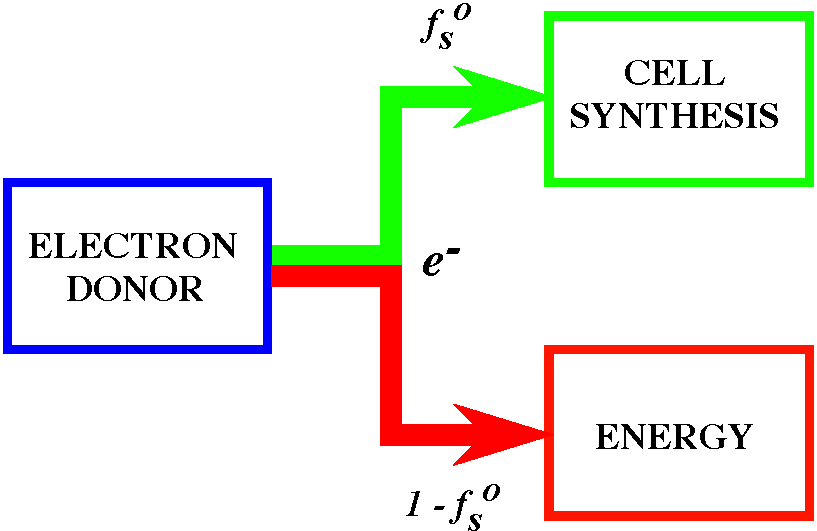
\includegraphics[scale=0.75]{figs/electrons}
\parbox{14cm}{\caption{
Schematic diagram illustrating the partitioning of electrons from the donor substrate to form biomass and create energy. 
}\label{feflow}} 
\end{figure} 

The transfer of electrons from the electron donor substrate must be conserved by cell processes of synthesis and respiration generating more biomass and energy. If the quantity $f_s^\circ$ represents the fraction of electrons going to biomass synthesis, then the fraction of electrons for respiration providing energy is 
\EQ
f_e^\circ \eq 1-f_s^\circ.
\EN
The flow of electrons from the donor substrate and their partitioning between biomass synthesis and energy production is illustrated in Figure~\ref{feflow}.
The overall reaction for biomass systhesis is constructed from a linear combination of reactions (\ref{donor}), (\ref{acceptor}) and (\ref{synthesis}) with weighting factors $f_s^\circ$ and $f_e^\circ$ (Christensen and McCarty, 1975; Pavlostathis and Giraldo-Gomez, 1991).
This may be accomplished by first writing these reactions in terms of a single electron brought to the right-hand side
\BA
\frac{1}{n_d^e} \A_d^{} - \frac{1}{n_d^e} \sum_j \nu_{jd}^{} \A_j^{} & \longrightarrow e^-, \label{donor1}\\
\frac{1}{n_a^e} \A_a^{} - \frac{1}{n_a^e} \sum_j \nu_{ja}^{} \A_j^{} & \arrows e^-, \label{acceptor1}\\
\frac{1}{n_c^e} \A_c^{}-\frac{1}{n_c^e} \sum_j \nu_{jc}^\S \A_j^{} & \longleftarrow e^-. \label{synthesis1}
\EA
Combining these reactions with weighting factors $f_s^\circ$ and $1-f_s^\circ$ according to
\EQ
\R_{(\ref{donor1})} - (1-f_s^\circ) \R_{(\ref{acceptor1})} - f_s^\circ \R_{(\ref{synthesis1})},
\EN
yields the following overall reaction for biomass synthesis
\EQ\label{overallbio}
\frac{1}{n_d^e} \A_d - \frac{1-f_s^\circ}{n_a^e} \A_a + \sum_j \left[ \frac{f_s^\circ}{n_c^e} \nu_{jc}^\S + \frac{1-f_s^\circ}{n_a^e} \nu_{ja}^{} - \frac{1}{n_d^e}\nu_{jd}^{} \right] \A_j \longrightarrow \frac{f_s^\circ}{n_c^e} \A_c.
\EN
From this reaction an expression for the yield $\Y_c^d$ for biomass synthesis is obtained as the ratio of the rate of cell production to the rate of donor substrate utilization
\EQ
\Y_c^d \eq f_s^\circ \dfrac{n_d^e}{n_c^e}.
\EN
The yield is proportional to the electron synthesis factor $f_s^\circ$ and the ratio of electrons transferred in the donor and biomass systhesis reactions.
The biomass yield may be different for different electron acceptor substrates as well.

With oxygen as the electron acceptor substrate, and taking $f_s^\circ \!\!=\!\! 0.64$, $n_c^e \!\!=\!\! 20$, $n_d^e \!\!=\!\! 18$, and $n_a^e \!\!=\!\! -4$, reaction (\ref{overallbio}) becomes
\BA\label{oxy}
&\rm 0.0555556 \, C_6H_9O_6N - 0.173333 \, CO_{2(aq)} + 0.0235556 \, H^+ - 0.102667 \, H_2O \nonumber\\
&\rm - 0.0235556 \, NH_4^+ + 0.09 \, O_{2(aq)} \longrightarrow \rm 0.032 \, C_5H_7O_2N.
\EA
The yield $\Y$ has the value $\Y \!\!=\!\! 0.576$.
Using as electron acceptor NO$_3^-$ with $f_s^\circ \!\!=\!\! 0.62$ gives
\BA\label{nit}
& \rm 0.0555556 \, C_6H_9O_6N - 0.178333 \, CO_{2(aq)} + 0.100556 \, H^+ - 0.142667 \, H_2O \nonumber\\
&- \rm 0.038 \, N_2 - 0.0245556 \, NH_4^+ + 0.076 \, NO_3^- \longrightarrow \rm 0.031 C_5H_7O_2N.
\EA
For this reaction the yield $\Y$ has the value $\Y \!\!=\!\! 0.558$.

Reactions (\ref{oxy}) and (\ref{nit}) are linearly independent provided the intra-cell electron synthesis factor $f_s^\circ$ is different for different electron acceptors. Otherwise the reactions are linearly dependent. Provided local equilibrium prevails within the aqueous phase between different redox couples, catalyzed by bacteria, reactions based on different electron-acceptor substrates with equal intra-cell electron factors $f_s^\circ$ are linearly dependent and as a consequence the stoichiometry of the linearly-dependent reactions does not play a role in the transport equations, their rates being additive [see Eqn.(\ref{parallelj})]. Only if disequilibrium of redox couples persists does the stoichiometry of the overall reaction come into play according to Eqn.(\ref{parallelkk}). 

\textbf{\textsl{Kinetic Rate Law.}} Introducing the yield, reaction (\ref{overallbio}) can be written as
\EQ\label{overally}
\frac{1}{\Y_c^d} \, \A_d - \frac{1-f_s^\circ}{f_s^\circ} \, \frac{n_c^e}{n_a^e} \, \A_a + \sum_j \left[ \nu_{jc}^\S + \frac{1-f_s^\circ}{f_s^\circ} \, \frac{n_c^e}{n_a^e} \, \nu_{ja}^{} - \frac{1}{\Y_c^d} \, \nu_{jd}^{} \right] \A_j \longrightarrow \A_c,
\EN
in which the stoichiometric coefficient multiplying biomass is normalized to unity.
The kinetic rate law for biomass synthesis is presumed to be adequately described by the Monod rate law
\EQ
I_c \eq k_c \, \chi_c \, \frac{C_d}{K_d + C_d} \, \frac{C_a}{K_a + C_a},
\EN
for single acceptor and donor substrates with concentrations $C_a$ and $C_d$, respectively, and where $k_c$ represents the rate constant and $\chi_c$ denotes the concentration of cells. Note that an affinity factor, present in mineral precipitation and dissolution reactions, is absent from the Monod rate law.
The rate law describing biomass decay is assumed to be first order of the form
\EQ
I_c^\D \eq - \lambda_c \chi_c,
\EN
where $\lambda_c$ denotes the decay constant.

\textbf{\textsl{Mass Transport Equations.}} To set up the mass transport equations the first step is to identify an appropriate set of primary and secondary species to represent the reactions taking place in the particular system at hand. The primary electron donor substrate must be chosen as primary species as well as at least one on the primary electron acceptor substrates. If redox reactions are described through kinetic rate laws then all electron acceptors become primary species. On the other hand if redox reactions are represented by local equilibrium constraints, catalyzed by the presence of bacteria, then only one electron acceptor can be chosen as primary species, with the remaining electron acceptors included as aqueous secondary species.
In addition to the biomass synthesis reaction (\ref{overally}) and decay reaction (\ref{decay}), and possibly electron acceptor equilibria, additional reactions including homogeneous reactions
\EQ
\nu_{di}^{aq} \A_d^{} + \nu_{ai}^{aq} \A_a^{} + \sum_j \nu_{ji}^{aq} \A_j^{} \arrows \A_i^{},
\EN
and mineral precipitation and dissolution reactions
\EQ
\nu_{di}^{min} \A_d^{} + \nu_{ai}^{min} \A_a^{} + \sum_j \nu_{jm}^{min} \A_j^{} \arrows \M_m^{},
\EN
must also be accounted for in a geochemical system. In these reactions allowance is made for participation by both the electron donor and acceptor substrates.
For the set of primary species $\{ \A_d, \ \A_a, \ \A_j \}$, the mass transport equations have the following form for primary species
\BA
\L C_d &\eq -\frac{1}{\Y_c^d} \, I_c^\S -\sum_i \nu_{di}^{aq} I_i^{aq} -\sum_m \nu_{dm}^{min} I_m^{min},\\
\L C_a &\eq \frac{1-f_s^\circ}{f_s^\circ} \, \frac{n_c^e}{n_a^e} \, I_c^\S + \nu_{ac}^\D \, \lambda_c \, \chi_c -\sum_i \nu_{ai}^{aq} I_i^{aq} -\sum_m \nu_{am}^{min} I_m^{min},\\
\L C_j &\eq -\left[ \nu_{jc}^\S + \frac{1-f_s^\circ}{f_s^\circ} \, \frac{n_c^e}{n_a^e} \, \nu_{ja} - \frac{1}{\Y_c^d} \, \nu_{jd} \right] I_c^\S +\nu_{jc}^\D \, \lambda_c \, \chi_c\nonumber\\
& \quad\quad\quad - \sum_i \nu_{ji}^{aq} I_i^{aq} -\sum_m \nu_{jm}^{min} I_m^{min},\\
\intertext{secondary species}
\L C_i &\eq I_i^{aq},\\
\intertext{biomass}
\frac{\p \chi_c}{\p t} &\eq I_c^\S - \lambda_c \chi_c,\\
\intertext{and finally for minerals}
\frac{\p \phi_m}{\p t} &\eq \bar V_m I_m^{min}.
\EA
Mineral reaction rates are denoted by $I_m^{min}$, and homogeneous aqueous reaction rates by $I_i^{aq}$. 

For the case in which the rates $I_i^{aq}$ for homogeneous reactions are in local equilibrium, their rates may be eliminated by replacing the corresponding transport equations with mass action equations. This results in the primary species transport equations
\seteqn
\BA
\L \Psi_d &\eq -\frac{1}{\Y_c^d} \, I_c^\S -\sum_m \nu_{dm}^{min} I_m^{min},\\
\L \Psi_a &\eq \frac{1-f_s^\circ}{f_s^\circ} \, \frac{n_c^e}{n_a^e} \, I_c^\S + \nu_{ac}^\D \, \lambda_c \, \chi_c -\sum_m \nu_{am}^{min} I_m^{min},\\
\L \Psi_j &\eq -\left[ \nu_{jc}^\S + \frac{1-f_s^\circ}{f_s^\circ} \, \frac{n_c^e}{n_a^e} \, \nu_{ja} - \frac{1}{\Y_c^d} \, \nu_{jd} \right] I_c^\S + \nu_{jc}^\D \, \lambda_c \, \chi_c -\sum_m \nu_{jm}^{min} I_m^{min},
\EA
\reseteqn
where
\seteqn
\BA
\Psi_d &\eq C_d + \sum_i \nu_{di}^{aq} C_i,\\
\Psi_a &\eq C_a + \sum_i \nu_{ai}^{aq} C_i,\\
\Psi_j &\eq C_j + \sum_i \nu_{ji}^{aq} C_i.
\EA
\reseteqn

\textbf{\textsl{Parallel Reactions.}} So far the discussion has focused on the presence a single electron donor and acceptor substrate. However, in natural systems it is common for a number of different electron donor and acceptor substrates to be present at any one time. In such cases several parallel reactions representing biosynthesis may take place simultaneously. For the case of multiple electron acceptors indexed by $\beta$, these reactions may be written collectively in the general form
\EQ
\sum_j \nu_{jc}^\beta \A_j \longrightarrow \A_c,
\EN
where the sum over the index $j$ includes electron donor and acceptor substrates in addition to the other primary species. The reaction rate is given by the Monod rate law
\EQ
I_c^\beta \eq k_c^\beta \chi_c \frac{C_{a_\beta^{}}}{K_{a_\beta^{}} + C_{a_\beta^{}}} \frac{C_d}{K_d + C_d},
\EN
with electron acceptor concentration $C_{a_\beta^{}}$. The total rate for biomass synthesis is given by the sum over all parallel reactions related to different electron acceptors
\BA
I_c &= \sum_\beta I_c^\beta,\nonumber\\
&= \chi_c \frac{C_d}{K_d + C_d} \sum_\beta \frac{k_c^\beta \, C_{a_\beta^{}}}{K_{a_\beta^{}} + C_{a_\beta^{}}}
\EA
For example, for parallel reactions based on O$_{2(aq)}$ and NO$_3^-$ as electron acceptors the total rate for biomass synthesis is equal to the sum of the individual rates
\BA
I_c &= I_{\rm O_{2(aq)}} + I_{\rm NO_3^-}, \nonumber\\
&= \chi_c \, \frac{C_d}{K_d + C_d} \, \left[ \frac{k_{\rm O_{2(aq)}} \, C_{\rm O_{2(aq)}}}{K_{\rm O_{2(aq)}} + C_{\rm O_{2(aq)}}} + \frac{k_{\rm NO_3^-} \, C_{\rm NO_3^-}}{K_{\rm NO_3^-} + C_{\rm NO_3^-}} \right].
\EA

The primary species mass transport equations can be written in the form
\EQ
\L \Psi_j \eq - \sum_{c\beta} \nu_{jc}^\beta I_c^\beta - \sum_{jm} \nu_{jm} I_m^{min},
\EN
and for biomass synthesis as
\EQ
\frac{\p \chi_c}{\p t} \eq \sum_\beta I_c^\beta \eq I_c.
\EN
The equations may be further generalized to more than one electron donor substrate if desired.

\section{Pitzer Activity Coefficient Algorithm}

\setcounter{equation}{0}

\section{Species-Dependent Diffusion}

\setcounter{equation}{0}

\subsection{Species-Independent Diffusion Coefficients}

For the case of species-independent diffusion coefficients, because the homogeneous and heterogeneous reactions conserve charge, expressed by Eqn.\eqref{chrg},
the mass conservation equations also conserve charge. The total charge density $\rho_e$ in solution must vanish
\EQ\label{electroneutrality}
\rho_e \eq \F\sum_jz_j\Psi_j\eq \F\sum_jz_jC_j+\F\sum_iz_iC_i \eq 0,
\EN
where $\F$ denotes the Faraday constant (96,485.3415 Coulombs/mol).
Multiplying the primary species transport equations Eqn.\eqref{pri} by $z_j$ and summing over all primary species noting that $\sum_{jm}z_j\nu_{jm}I_m=\sum_mz_mI_m=0$ from Eqn.\eqref{chrg}, gives
\EQ
\frac{\p}{\p t}\varphi\rho_e + \bnabla\bdot\bOmega_{\rho_e} \eq 0,
\EN
where $\bOmega_{\rho_e}$ is defined as
\EQ
\bOmega_{\rho_e} \eq \big(\bq - \varphi\bD\!\bdot\!\bnabla\big)\rho_e.
\EN
Thus the flux can be expressed in terms of $\rho_e$ alone, and therefore if $\rho_e=0$ initially, it must remain zero as the system evolves in time.

\subsection{Species-Dependent Diffusion Coefficients}

Real aqueous electrolyte solutions consist of charged species that diffuse at different rates. This requires consideration of electrochemical effects on transport in order to maintain charge balance. For charged species the solute flux is obtained from the Nernst-Planck equation involving the sum of gradients of the chemical and electric potentials as (Newman, 1991)
%\EQ\label{eflux}
%\bF_i \eq - \tau \phi z_i \frac{D_i C_i}{RT} \F \bnabla \Phi - \tau 
%\phi D_i \big( \bnabla C_i + C_i \bnabla \ln \gamma_i \big) + {\bq} C_i,
%\EN
%\EQ\label{eflux}
%\bF_i \eq v_i^e C_i 
%- \tau \phi \frac{z_i D_i C_i}{RT} \bnabla \mu_i 
%+ {\bq} C_i,
%\EN
\EQ\label{eflux}
\bF_i \eq - \tau \phi \frac{D_i C_i}{RT} \bnabla \big(\mu_i +\F z_i\Phi\big)
+ {\bq} C_i,
\EN
where  chemical potential $\mu_i$ [J/mol] is defined by
\EQ
\mu_i\eq\mu_i^\circ(T,\,p) + RT\ln \gamma_i C_i,
\EN
with standard state potential $\mu_i^\circ(T,\,p)$, and the last term refers to bulk advective transport. Here $z_i$, $\gamma_i$ and $D_i$ denote the valence, 
activity coefficient and diffusivity of the $i$th species, 
respectively. The quantity $\Phi$ [J/Coul] represents the electrical potential, $\F$ [Coul/mol] denotes the Faraday constant, $\tau$ refers to the 
tortuosity of the porous medium, and $\bf q$ denotes the Darcy fluid 
velocity. 

As is apparent from the form of the solute flux Eqn.\eqref{eflux}, electrochemical 
migration leads to a species-dependent velocity field $v_i^e$ superimposed on the bulk fluid flow, 
defined by
\EQ
v_i^e \eq - \tau \phi \frac{z_i D_i}{RT} \F \nabla \Phi.
\EN
The electrochemical velocity is proportional to the charge on the ion, the diffusivity and the electric potential gradient. The minus sign ensures that positively charged ions migrate in the direction of the electric field. Electrochemical effects may have several different origins. One possible contribution comes from diffusion of ionic species with differing diffusion coefficients. An electric field is established which acts on the charged species and influences their rates of migration in order to maintain electroneutrality of the aqueous solution. Another contribution is the electrochemical reaction of solids involving the transfer of electrons. Half-cell reactions are not in general balanced locally, but may occur at spatially distinct locations resulting in the formation of an electric current in both the aqueous solution and solid porous matrix. 

\begin{table}[t]\centering
\parbox{4.5in}{\caption{Tracer diffusion coefficients of ions at infinite dilution in deionized water at 25\degc\ (modified from Lasaga, 1998).}\label{tdiff}}

\vspace{5mm}

\begin{tabular}{lrlr}
\toprule
\multicolumn{2}{c}{Cations $D_i\!\times\! 10^5$ cm$^2$/s} & \multicolumn{2}{c}{Anions $D_i\!\times\! 10^5$ cm$^2$/s} \\
\midrule
H$^+$ & 9.31 & OH$^-$ & 5.27 \\
Li$^+$ & 1.03 & F$^-$ & 1.46 \\
Na$^+$ & 1.33 & Cl$^-$ & 2.03 \\
K$^+$ & 1.96 & Br$^-$ & 2.01 \\
Rb$^+$ & 2.06 & I$^-$ & 2.00 \\
Cs$^+$ & 2.07 & IO$_3^-$ & 1.06 \\
NH$_4^{+}$ & 1.98 & HS$^-$ & 1.73 \\
Ag$^+$ & 1.66 & HSO$_4^-$ & 1.33 \\
Mg$^{2+}$ & 0.705 & NO$_2^-$ & 1.91 \\
Ca$^{2+}$ & 0.793 & NO$_3^-$ & 1.90 \\
Sr$^{2+}$ & 0.794 & HCO$_3^-$ & 1.18 \\
Ba$^{2+}$ & 0.848 & H$_2$PO$_4^-$ & 0.846 \\
Mn$^{2+}$ & 0.688 & H$_2$AsO$_4^-$ & 0.905 \\
Fe$^{2+}$ & 0.719 & H$_2$SbO$_4^-$ & 0.825 \\
Co$^{2+}$ & 0.699 & SO$_4^{2-}$ & 1.07 \\
Ni$^{2+}$ & 0.679 & SeO$_4^{2-}$ & 0.946 \\
Cu$^{2+}$ & 0.733 & CO$_3^{2-}$ & 0.955 \\
Zn$^{2+}$ & 0.715 & HPO$_4^{2-}$ & 0.734 \\
Cd$^{2+}$ & 0.717 & CrO$_4^{2-}$ & 1.12 \\
Pb$^{2+}$ & 0.945 & MoO$_4^{2-}$ & 0.991 \\
UO$_2^{2+}$ & 0.426 & PO$_4^{3-}$ & 0.612 \\
Cr$^{3+}$ & 0.594 \\
Fe$^{3+}$ & 0.607 \\
Al$^{3+}$ & 0.559\\
\bottomrule
\end{tabular}
\end{table}

To account for effects of pH and aqueous complexing reactions it is necessary to allow for homogeneous equilibrium reactions with the possibility of charged secondary species. Note that from Table~\eqref{tdiff} the species H$^+$ and OH$^-$ have the largest tracer diffusion coefficients. It is assumed that homogeneous reactions are fast and local equilibrium conditions may be assumed. As for the case of equal diffusivities, it is also possible in the case of species-dependent diffusivities to derive mass conservation equations for the primary species taking into account homogeneous equilibrium relations. However, in this case it is no longer possible to express the primary species transport equations in terms of the total concentration $\Psi_j$ alone, but in this case each individual species now occurs in the transport equations. To derive the form of the primary species transport equations, first separate equations are written for primary and secondary species including rates of the homogeneous reactions $I_i$ as before [see Eqns.\eqref{eqpri} and \eqref{eqsec}], but with the solute flux $\bF_l$ now given by Eqn.\eqref{eflux}.
Substituting Eqn.\eqref{eflux} into Eqn.\eqref{omega}, the total primary species flux is found to be after rearranging terms
\BA
\bOmega_j \eq & -\tau\varphi\frac{\F\bnabla \Phi}{RT}\big(z_j D_j C_j + \sum_i\nu_{ji} z_i D_i C_i\big) 
\nonumber\\
&-\tau \varphi \left(D_j \bnabla C_j + \sum_i\nu_{ji} D_i \bnabla C_i\right.\nonumber\\
& + \left. D_j C_j \bnabla \ln \gamma_j + \sum_i\nu_{ji} D_i C_i \bnabla \ln \gamma_i \right) + {\bq} \Psi_j.
\EA
Defining the quantities
\EQ
\Lambda_j \eq z_j D_j C_j + \sum_i\nu_{ji} z_i D_i C_i,
\EN
\EQ
\Gamma_j^C \eq D_j \bnabla C_j + \sum_i\nu_{ji} D_i \bnabla C_i,
\EN
and
\EQ
\Gamma_j^\gamma \eq D_j C_j \bnabla \ln \gamma_j + \sum_i\nu_{ji} D_i C_i \bnabla \ln \gamma_i
\EN
the flux may be expressed in the more compact form
\EQ\label{eomega}
\bOmega_j\eq -\tau\varphi\left(\frac{\F\bnabla \Phi}{RT} \Lambda_j^{} + \Gamma_j^C + \Gamma_j^\gamma \right) + \bq \Psi_j.
\EN
It is possible to eliminate the potential $\Phi$ from the total flux by introducing the current density $\bi_e$ defined as
\EQ\label{current}
\bi_e\eq \F\sum_jz_j\bOmega_j.
\EN
Substituting for $\bOmega_j$ from Eqn.\eqref{eomega}, the current density becomes
\EQ\label{current2}
\bi_e \eq -\tau\varphi\F\left(\frac{\F\bnabla \Phi}{RT} \sum_jz_j\Lambda_j^{} + \sum_jz_j\big(\Gamma_j^C + \Gamma_j^\gamma\big) \right) + \bq\rho_e.
\EN
Assuming the aqueous solution is electrical neutral the last term vanishes according to Eqn.\eqref{electroneutrality}.
%\EQ\label{electroneutrality}
%\rho_e\eq\F\sum_jz_j \Psi_j\eq 0.
%\EN
Solving Eqn.\eqref{current2} for $\bnabla\Phi$ yields the expression
\EQ\label{pot}
\bnabla\Phi\eq -\frac{1}{\kappa}\left(\bi_e -\bq\rho_e + \tau\varphi\F\sum_j z_j\big(\Gamma_j^C + \Gamma_j^\gamma\big)\right),
\EN
where the conductivity 
%Debye length 
$\kappa$ is defined as
\EQ
\kappa \eq \frac{\tau\varphi\F^2}{RT}\sum_j z_j\Lambda_j^{}.
\EN
Note that the sum on the right-hand side can be simplified to
\EQ
\sum_{j=1}^{N_c}z_j^{}\Lambda_j^{}\eq \sum_{k=1}^N z_k^2 D_k^{} C_k^{},
\EN
using the identity $\sum_jz_j\nu_{ji}\!=\!z_i$, where the sum over $k$ includes all species, primary and secondary.
The solute flux $\bOmega_j$ may now be expressed in terms of the current $\bi_e$ as
\EQ\label{totflux}
\bOmega_j \eq \frac{t_j}{z_j\F} \big(\bi_e -\bq\rho_e\big) -\tau\varphi \sum_l\beta_{jl}^{}\big(\Gamma_l^C+\Gamma_l^\gamma\big) + \bq \Psi_j,
\EN
where the matrix $\beta_{jl}$ is a projection operator ($\bb^2\!=\!\bb$) defined by
\EQ
\beta_{jl}^{}\eq\delta_{jl}^{} - \frac{z_l^{}}{z_j^{}}\Upsilon_j^{},
\EN
with the property
\EQ
\sum_jz_j\beta_{jl} \eq 0,
\EN
and where the generalized transference number $\Upsilon_j$ is defined as
\EQ
\Upsilon_j \eq\frac{z_j\Lambda_j}{\displaystyle\sum_lz_l\Lambda_l}.
\EN

To demonstrate that charge is indeed conserved,
the primary species transport equations Eqn.\eqref{pri} with flux given by Eqn.\eqref{totflux} are multiplied by the valence $z_j$ and summed over all primary species to yield
\EQ\label{chrgcon}
\frac{\p}{\p t} \varphi\rho_e + \bnabla\bdot\bi_e\eq 0.
\EN
In order for the electroneutrality condition Eqn.\eqref{electroneutrality} to be satisfied, Eqn.\eqref{chrgcon} implies that the divergence of the current must vanish
\EQ
\bnabla\bdot\bi_e \eq 0,
\EN
which in turn requires that $\bi_e\!=\!\boldsymbol 0$. This will be the case if both $\rho_e$ and $\bi_e$ vanish initially. These results assume that corrosion processes which result in a source/sink term and nonzero current are not applicable.

\section{Multiple Interacting Continua}

\setcounter{equation}{0}

A fundamental problem facing efforts to model subsurface reactive flows is characterizing and incorporating a multitude of spatial scales that are typical of natural systems into multi\-com\-po\-nent-multiphase numerical models. Spatial scales may range from nanoscale surface chemistry, to pore and fracture apertures of millimeters to centimeters, to fracture spacing and matrix block sizes of tens of centimeters to meters, to reservoir or basin scales of kilometers to tens of kilometers. To illustrate the technical challenges involved in modeling multi-scale subsurface processes, consider a basin scale reservoir with an areal extent of one square kilometer and depth of 500 meters. Modeling this system as a single continuum on a grid with one million nodes results in an average grid block size of 10m by 10m by 5m---or roughly the size of a large conference room. Within this grid block, physical and chemical processes occur at much smaller sub-grid scales. Such processes involve, for example, diffusive and advective mass transfer between fractures and rock matrix, or more generally diffusion between macro- and micro-pore scales, accompanied by chemical reactions. Characteristic of these systems is mass transport and chemical reactions occurring at disparate spatial scales that cannot be captured within a single continuum description. In particular, localized chemical environments may be vastly different from the bulk fluid and lead to dramatically different results compared to a single continuum description. It is clearly impossible to capture this range of scales within a single continuum framework because of the large computational expense that would be required to resolve the smallest scale. One approach that appears feasible to describe such systems is to incorporate sub-grid scale processes through multiple interacting continua representing fine scale processes. Besides the difficulty developing conceptual models of such systems, characterization at the laboratory and field scales adds additional challenges. In addition, this approach carries a significant computational cost as well because of the increase in the number of degrees of freedom associated with the additional continua and the necessity to carry out calculations over engineering and geologic time spans within feasible computation times. 

A considerable body of literature exists on multiscale descriptions of flow and transport in porous and fractured media. Such formulations range from structured soils (Murphy et al., 1986; van Genuchten and Wagenet, 1989; Brusseau and Rao, 1990; Gerke and van Genuchten, 1993; Gwo et al., 1995; and others), to fractured rock (Warren and Root, 1956; Barenblatt et al., 1960; Duguid and Lee, 1977; Pruess and Narisimhan, 1985; Bai et al., 1993; Lichtner, 2000).
These works, however, have been largely confined to consideration of flow and simple single component systems with first order linear kinetics or a constant $K_D$ model.
Precipitation and dissolution reactions which result in a moving boundary problem associated with different mineral assemblages are usually not included in the description. 

In the soil science literature these models are referred to as two-site and two-domain, or more generally multi-site and multi-domain models, and have been generalized to so-called multi-rate models by Haggerty and Gorelick (1995). In fractured rock studies, they have various names including dual permeability-dual porosity models or more generally dual and multiple continuum models. They may involve both saturated and partially saturated conditions.

Distinguishing between different domains is somewhat arbitrary and nonunique especially in soils (Lichtner and Kang, 2007). Which pores participate in flow depends on the degree of saturation of the medium. A typical approach is to divide pores into macro pores which carry the bulk fluid and micro pores which are connected to macro pores by diffusion. Inter- (between macro pores) and intra- (inside micro pores) mass transfer between the different pores is formulated as a set of coupled partial differential equations based on the generalization of a single continuum to interacting continua.

One of the primary difficulties in applying a multiscale formulation is obtaining values for the parameters that enter into the model. As has been demonstrated for linear single component systems these values may be nonunique (Sardin et al., 1991).

Multiscale processes play a significant role in many situations involving flow and reactive transport. However, because of the inherent nonlinearity of constitutive relations, for example, chemical rate laws and statements of equilibrium mass action relations in real multicomponent fluids, use of linear relations is of limited usefulness.

The formulation presented below is based on a multiple interacting continuum formulaiton. This formulation provides for local concentration gradients within a sub-continuum domain. The model places no restrictions on linear or nonlinear constitutive relations, and is completely general in its treatment of chemical and other physical processes.

In the following a multi-scale continuum formulation for reactive transport is developed based on multiple interacting continua. In this formulation the primary continuum, which may consist of one, two, or three spatial dimensions, is coupled to sub-grid scale domains that are presumed to form effective one-dimensional regions. 
%The sub-grid domains are coupled only to the primary continuum and not to each other as illustrated in Figure~\ref{F:subgrid} which shows the connectivity between primary and secondary continua. 

A control, or representative elemental volume $V$ of the porous medium is subdivided into regions consisting of primary and secondary continua. A single volume is associated with the primary continuum although this assumption could be relaxed. The geometry of the system is assumed to be characterized by the primary continuum volume fraction $\epsilon_\a$, the intrinsic volume and surface area of each secondary continuum domain $V_\b^0$ and $A_\b^0$, respectively, and the fraction $x_\b$ of the number of the $\b$th subdomain type
\EQ
x_\b\eq\frac{N_\b}{N},
\EN
where $N$ is the total number of secondary domains in a control volume and $N_\b$ is the number of subdomains of type $\b$. The total volume $V$ may thus be represented as
\EQ
V\eq V_\a+\sum_\b V_\b,
\EN
where the sum is over all secondary continua with volume $V_\b$ expressed as
\EQ
V_\b^{}\eq N_\b^{} V_\b^0,
\EN
in terms of the volume $V_\b^0$ of a particular type and the number of such types within a control volume. The primary continuum volume fraction $\epsilon_\a$ is related to the number density of secondary domains by the expression
\EQ
\epsilon_\a \eq \frac{V_\a}{V}\eq 1-\frac{1}{V}\sum_\b N_\b^{} V_\b^0,
\EN
or
\EQ
\frac{N}{V}\eq \frac{1-\epsilon_\a}{\displaystyle\sum_\b x_\b^{} V_\b^0}.
\EN
The volume fraction $\epsilon_\b$ of each secondary continuum is given by
\EQ
\epsilon_\b \eq \big(1-\epsilon_\a\big) \frac{x_\b^{} V_\b^0}{\displaystyle\sum_{\b'} x_{\b'}^{} V_{\b'}^0}.
\EN
Also of interest is the specific interfacial surface area $a_{\a\b}$ separating primary and secondary continua
\EQ
a_{\a\b} \eq \frac{A_{\a\b}}{V} \eq \frac{1}{V}\sum_\b N_\b^{} A_\b^0 \eq \big(1-\epsilon_\a\big) \frac{x_\b^{} A_\b^0}{\displaystyle\sum_{\b'} x_{\b'}^{} V_{\b'}^0}.
\EN

Multi-scale, multicomponent, continuum-scale reactive transport equations for primary species $\A_j$ participating in reactions given in Eqns.\eqref{rxnleq} and \eqref{rxnhet} can be written in the general form as the set of coupled partial differential equations as follows (Lichtner and Kang, 2007)
\BA\label{bulk}
\frac{\p}{\p t} \epsilon_\a\varphi_\a \Psi_j^\a + \bnabla\bdot\bOmega_j^\a \eq \sum_\b a_{\a\b}^{} \Omega_j^{\a\b} - \epsilon_\a\sum_{s} \nu_{js}^{} I_{s}^\a,
\EA
for the primary continuum fluid, and
\BA\label{matrix}
\frac{\p}{\p t} \varphi_\b \Psi_j^\b &+ \bnabla\bdot\bOmega_j^\b \eq  - \sum_s \nu_{js}^{} I_s^\b,
\EA
for the $\b$th sub-grid domain. The quantity $\epsilon_\a$ represents the volume fraction occupied by the primary continuum. The volume averaged kinetic mineral reaction rate $I_s^{\a,\b}$ has the form
\EQ
I_s^{\a,\b}\eq -k_s^{\a,\b} a_s^{\a,\b} (1-K_s Q_s^{\a,\b}),
\EN
with rate constant $k_s^{\a,\b}$ and mineral surface area $a_s^{\a,\b}$ for primary continuum $\a$ and sub-grid continua $\b$.
The total concentration $\Psi_j^{\a,\,\b}$ is given by Eqn.\eqref{psi} for the primary and secondary continua. The total solute flux includes advective and diffusive terms
\EQ
\bOmega_j^{\a,\b} \eq -\varphi_{\a,\b}^{}\tau_{\a,\b}^{} D\bnabla \Psi_j^{\a,\b} + \bq_{\a,\b}^{} \Psi_j^{\a,\b},
\EN
with tortuosity $\tau_{\a,\b}$, diffusivity $D$, and Darcy flow rate $\bq_{\a,\b}$. For simplicity dispersion is not included, but in general would be necessary. 
%Note that Eqn.\eqref{bulk} is referenced to the bulk volume, including both primary continuum and sub-grid domains, whereas Eqn.\eqref{matrix} is referenced to the sub-grid domain volume, whence the factor $\epsilon_\a$ appears only in Eqn.\eqref{bulk}.

The boundary condition at the primary continuum-matrix fluid interface is given by
\EQ
C_j^\b(r=r_\b,\, t; \br) \eq C_j^\a(\br,\,t),
\EN
where $r_\b$ denotes the boundary of the domain $\b$.
The flux at the primary continuum-matrix interface is presumed to only involve diffusion with the form
\EQ
\Omega_j^{\a\b} \eq -\varphi_\b \tau_\b D \,\bn_\b\bdot\bnabla \Psi_j^\b\bigg|_{r_\b},
\EN
where $\bn_\b$ denotes the outward normal to the interface.
The matrix equation is quite general and applies to various geometries including spheres and linear domains. As an approximation cubes and irregular shaped domains may be used. Because of computational considerations, the sub-grid domain equations are reduced to an equivalent 1D problem. 
For further discussion of numerical techniques for efficiently solving the multi-scale equations see Lichtner (2006).

\section{Electrical Conductivity}

\section{Hydration-Dehydration Reactions}

\section{Multiphase Systems}

For a multiphase system characterized with phase saturation $s_\a$, and Darcy velocity $\bq_\a$ the transport equations generalize to
\EQ
\frac{\p}{\p t}\left(\varphi\sum_\a s_\a\Psi_j^\a\right) + \bnabla\cdot\sum_\a\bOmega_j^\a \eq \R_j,
\EN
where $s_\a$ denotes the saturation of phase $\a$, $\R_j$ refers to source/sink and reaction rate terms, and the total concentration for each phase is defined as
\EQ
\Psi_j^\a \eq \delta_{l\a} C_j^l + \sum_i\nu_{ji}^\a C_i^\a.
\EN
The total flux (for species-independent diffusion) is given by
\EQ
\bOmega_j^\a \eq \bq_\a \Psi_j^\a -\varphi s_\a D_\a \bnabla \Psi_j^\a,
\EN
for diffusion/dispersion coefficient $D_\a$, Darcy velocity $\bq_a$ defined in terms of relative permeability $k_\a$ as
\EQ
\bq_\a \eq \frac{kk_\a}{\mu_\a}\bnabla(p_\a -\rho_\a \bg z),
\EN
with bulk permeability $k$, fluid density $\rho_\a$, and acceleration of gravity $\bg$. The fluid pressure $p_\a$ satisfies the relations
\EQ
p_\a-p_\b \eq p_{\a\b}^c,
\EN
for capillary pressure $p_{\a\b}^c$.

The Kronecker delta function appears in the expression for the total concentration $\Psi_j^\a$ multiplying the primary species concentration because it is assumed that all primary species belong to the aqueous phase. This condition could be relaxed, but it would require introducing variable switching at phase boundaries where phase changes take place. In the current implementation, if the aqueous phase completely disappears it is necessary to ``freeze'' the total aqueous concentration at some arbitrarily chosen minimum threshold value for the liquid saturation $s_l^{\rm min}$:  $(s_l^{}\!\leq\!s_l^{\rm min})$. If the system resaturates $(s_l^{}\!>\!s_l^{\rm min})$, this ``frozen'' total aqueous concentration must be released back into the system.

The residual function has the form
\EQ
R_{jn}\eq\frac{V_n}{\Delta t}\left[\bigg(\varphi_n\sum_\a s_{\a n} \Psi_{jn}^\a\bigg)_{t+\Delta t} - \bigg(\varphi_n\sum_\a s_{\a n} \Psi_{jn}^\a\bigg)_{t}\right] + \sum_{\a n'}\Omega_{jnn'}^\a A_{nn'} -\R_{jn} V_n.
\EN

\section{Stress-Strain Relations}

The functional relation of porosity to pore compressibility $c_{rp}$ and expansibility $c_{rT}$ is assumed to have the form
\EQ
\varphi \eq \varphi_{0} \big[1+c_{rp} (p-p_{0})-c_{rT} (T-T_{0})\big],
\EN
for reference state $\varphi_0$, $p_0$ and $T_0$. It follows that
\begin{align}\label{dpor}
\delta \phi &= \varphi_{0} c_{rp} \delta p - \varphi_{0} c_{rT} \delta T,\nonumber\\
&= \varphi_p \delta p + \varphi_T \delta T,
\end{align}
where $\varphi_p$ and $\varphi_T$ are derivatives with respect to pressure and temperature, respectively, and compressivity and thermal expansivity are defined by
\EQ
c_{rp} \eq \frac{1}{\varphi} \frac{\p \varphi}{\p p},
\EN
and
\EQ
c_{rT} \eq -\frac{1}{\varphi} \frac{\p \varphi}{\p T}.
\EN
As defined, both quantities $c_{rp}$ and $c_{rT}$ are positive for normal materials.

\section{Global Mass Conservation}

Taking the transport equations in the form
\EQ
\frac{\p}{\p t} \left[ \varphi \sum_\a s_\a \Psi_j^\a +\sum_k\nu_{jk} S_k\right] + \bnabla\cdot\sum_\a\bOmega_j^\a \eq -\sum_m\nu_{jm}I_m,
\EN
with
\EQ
\frac{\p\varphi_m}{\p t} \eq \overline V_m I_m,
\EN
global mass conservation equations are obtained by integrating over the computational domain $V$ with bounding surface $\p V$ to give
\EQ
\frac{d}{dt}\int_V \left[\varphi \sum_\a s_\a \Psi_j^\a +\sum_k\nu_{jk} S_k + \sum_m \overline V_m^{-1} \varphi_m \right] dV \eq -\sum_\a\int_{\p V} \bOmega_j^\a \cdot \bdS.
\EN
Defining $N_j$ equal to the total mass in place at time $t$ as
\EQ
N_j (t)\eq\int_V \left[\varphi \sum_\a s_\a \Psi_j^\a + \sum_k\nu_{jk} S_k + \sum_m \overline V_m^{-1} \varphi_m \right] dV,
\EN
gives
\EQ
\frac{dN_j}{dt} \eq -\sum_\a\int_{\p V} \bOmega_j^\a \cdot \bdS.
\EN
Integrating over time then yields
\EQ
N_j(t)\eq N_j(0) -\sum_\a\int_0^t dt \int_{\p V} \bOmega_j^\a \cdot \bdS.
\EN
Finally, defining $\G_j^\a(t)$ as the cumulative mass entering and leaving the system
\EQ
\G_j^\a(t) \eq \int_0^t dt \int_{\p V} \bOmega_j^\a \cdot \bdS,
\EN
the global mass conservation equation becomes
\EQ
N_j(t) + \sum_\a\G_j^\a(t)\eq N_j(0).
\EN


\section{References}

\end{document}
%
\begin{comment}
\begin{subequations}
\BA
R_{jn}^{\rm ex} &\eq \frac{V_n}{z_j}\sum_{i\ne j} I_{ji,n},\\
R_{in}^{\rm ex} &\eq -\frac{V_n}{z_i} I_{ji,n},
\EA
\end{subequations}
\end{comment}
%

%
\begin{comment}
The contribution of ion exchange to the Jacobian matrix has the following forms for the reference cation
\begin{subequations}
\BA
\frac{\p R_{jn}^{\rm ex}}{\p\ln C_{jn}} &\eq -\frac{V_n}{z_j}C_{jn}\sum_{i\ne j} \frac{\p I_{ji,n}}{\p C_{jn}},\\
\frac{\p R_{jn}^{\rm ex}}{\p\ln C_{in}} &\eq -\frac{V_n}{z_j} C_{in}\frac{\p I_{ji,n}}{\p C_{in}},\\
\frac{\p R_{jn}^{\rm ex}}{\p S_{jn}} &\eq -\frac{V_n}{z_j}\sum_{i\ne j} \frac{\p I_{ji,n}}{\p S_{jn}},\\
\frac{\p R_{jn}^{\rm ex}}{\p S_{in}} &\eq -\frac{V_n}{z_j} \frac{\p I_{ji,n}}{\p S_{in}},
\EA
\end{subequations}
and for all other cations
\begin{subequations}
\BA
\frac{\p R_{in}^{\rm ex}}{\p\ln C_{jn}} &\eq \frac{V_n}{z_i} C_j\frac{\p I_{ji,n}}{\p C_{jn}},\\
\frac{\p R_{in}^{\rm ex}}{\p\ln C_{in}} &\eq \frac{V_n}{z_i} C_i\frac{\p I_{ji,n}}{\p C_{in}},\\
\frac{\p R_{in}^{\rm ex}}{\p S_{jn}} &\eq \frac{V_n}{z_i} \frac{\p I_{ji,n}}{\p S_{jn}},\\
\frac{\p R_{in}^{\rm ex}}{\p S_{in}} &\eq \frac{V_n}{z_i} \frac{\p I_{ji,n}}{\p S_{in}}.
\EA
\end{subequations}
\end{comment}

%
\begin{comment}
Sorbed concentrations give
\begin{subequations}
\BA
\frac{\p R_{N_{\rm ex}+j,n}}{\p\ln C_{jn}} &\eq \frac{V_n}{z_j}C_j\sum_{i\ne j} \frac{\p I_{ji,n}}{\p C_{jn}},\\
\frac{\p R_{N_{\rm ex}+j,n}}{\p\ln C_{in}} &\eq \frac{V_n}{z_j} C_i\frac{\p I_{ji,n}}{\p C_i},\\
\frac{\p R_{N_{\rm ex}+j,n}}{\p S_{jn}} &\eq \frac{V_n}{\Delta t} - \frac{V_n}{z_j}\sum_{i\ne j} \frac{\p I_{ji,n}}{\p S_{jn}},\\
\frac{\p R_{N_{\rm ex}+j,n}}{\p S_{in}} &\eq \frac{V_n}{\Delta t} - \frac{V_n}{z_j} \frac{\p I_{ji,n}}{\p S_i},
\EA
\end{subequations}
\begin{subequations}
\BA
\frac{\p R_{N_{\rm ex}+i,n}}{\p\ln C_{jn}} &\eq \frac{V_n}{z_i} C_j\frac{\p I_{ji,n}}{\p C_{jn}},\\
\frac{\p R_{N_{\rm ex}+i,n}}{\p\ln C_{in}} &\eq \frac{V_n}{z_i} C_i\frac{\p I_{ji,n}}{\p C_{in}},\\
\frac{\p R_{N_{\rm ex}+i,n}}{\p S_{jn}} &\eq \frac{V_n}{\Delta t} + \frac{V_n}{z_i} \frac{\p I_{ji,n}}{\p S_{jn}},\\
\frac{\p R_{N_{\rm ex}+i,n}}{\p S_{in}} &\eq \frac{V_n}{\Delta t} + \frac{V_n}{z_i} \frac{\p I_{ji,n}}{\p S_{in}}.
\EA
\end{subequations}
\end{comment}
%

\begin{comment}
\noindent Conversion to Mass Units (mol/dm$^3$ $\rightarrow$ mol/g)
\EQ
S_j^M \eq \frac{\overline N_j}{M_s} \eq \frac{\overline N_j}{V} \frac{V}{V_s} \frac{V_s}{M_s} \eq \frac{S_j}{(1-\varphi)\rho_s}
\EN
\EQ
{\rm CEC} \eq \frac{N_{\rm sites}}{M_s} \eq \frac{N_{\rm sites}}{A_s} \frac{A_s}{M_s} \eq \zeta_s \A_s
\EN
\end{comment}
